\documentclass[11pt, a4paper]{article}

\usepackage[a4paper, margin=2cm]{geometry}
\usepackage{setspace}
\usepackage[portuguese]{babel}
\usepackage{graphicx}
\usepackage{hyperref}
\usepackage{amsfonts}
\usepackage[dvipsnames]{xcolor}
\usepackage{float}
\usepackage{footnote}

\chardef\_=`_

\title{\textbf{LI3 - Relatório da Fase II - Grupo 12}}
\author{
    Humberto Gomes (A104348) \\
    José Lopes     (A104541) \\
    José Matos     (A100612) \\
}
\date{janeiro de 2024}

\makesavenoteenv{tabular}
\begin{document}

\maketitle
\onehalfspacing
\setlength{\parskip}{\baselineskip}
\setlength{\parindent}{0pt}

\pagebreak
\begin{abstract}
    Após a entrega da primeira fase deste trabalho, procurámos implementar as funcionalidades em
    falta para a conclusão do desenvolvimento desta aplicação: as restantes quatro \emph{queries},
    um modo de uso interativo (uma interface TUI), testes funcionais e de desempenho, e suporte
    para um \emph{dataset} de maior dimensão, mantendo um desempenho aceitável. Adicionalmente,
    procurámos também melhorar o encapsulamento e a modularidade no nosso projeto.
\end{abstract}

\section{Estrutura do trabalho}

Nesta secção, procuramos descrever as diferenças entre a nossa arquitetura atual e a que tínhamos
na primeira fase do projeto. Devido ao elevado número de módulos, dividimos a aplicação em
subsistemas, que são descritos e esquematizados um a um. Nesses esquemas, para reduzir a
complexidade visual, não incluímos todas as relações de dependência, mas apenas as mais relevantes.
Segue-se a nossa convenção gráfica:

\begin{itemize}
    \item Um retângulo com cantos arredondados representa uma estrutura de dados (entidades,
          gestores, \ldots);
    \item Um retângulo sem cantos arredondados representa um módulo cuja tarefa principal é a
          execução de código. Mesmo assim, alguns destes módulos podem conter estruturas de dados
          auxiliares (por exemplo, uma gramática definida no módulo de um \emph{parser});
    \item $A \rightarrow B$ significa que o módulo $A$ depende do módulo $B$.
    \item Qualquer módulo ou relação de dependência representado(a) a {\color{ForestGreen}verde}
          indica que o(a) mesmo(a) é uma adição nesta segunda fase, ausente na entrega anterior.
\end{itemize}

\subsection{\emph{Parsing}}
\label{sec:parsing}

\begin{figure}[ht]
    \centering
    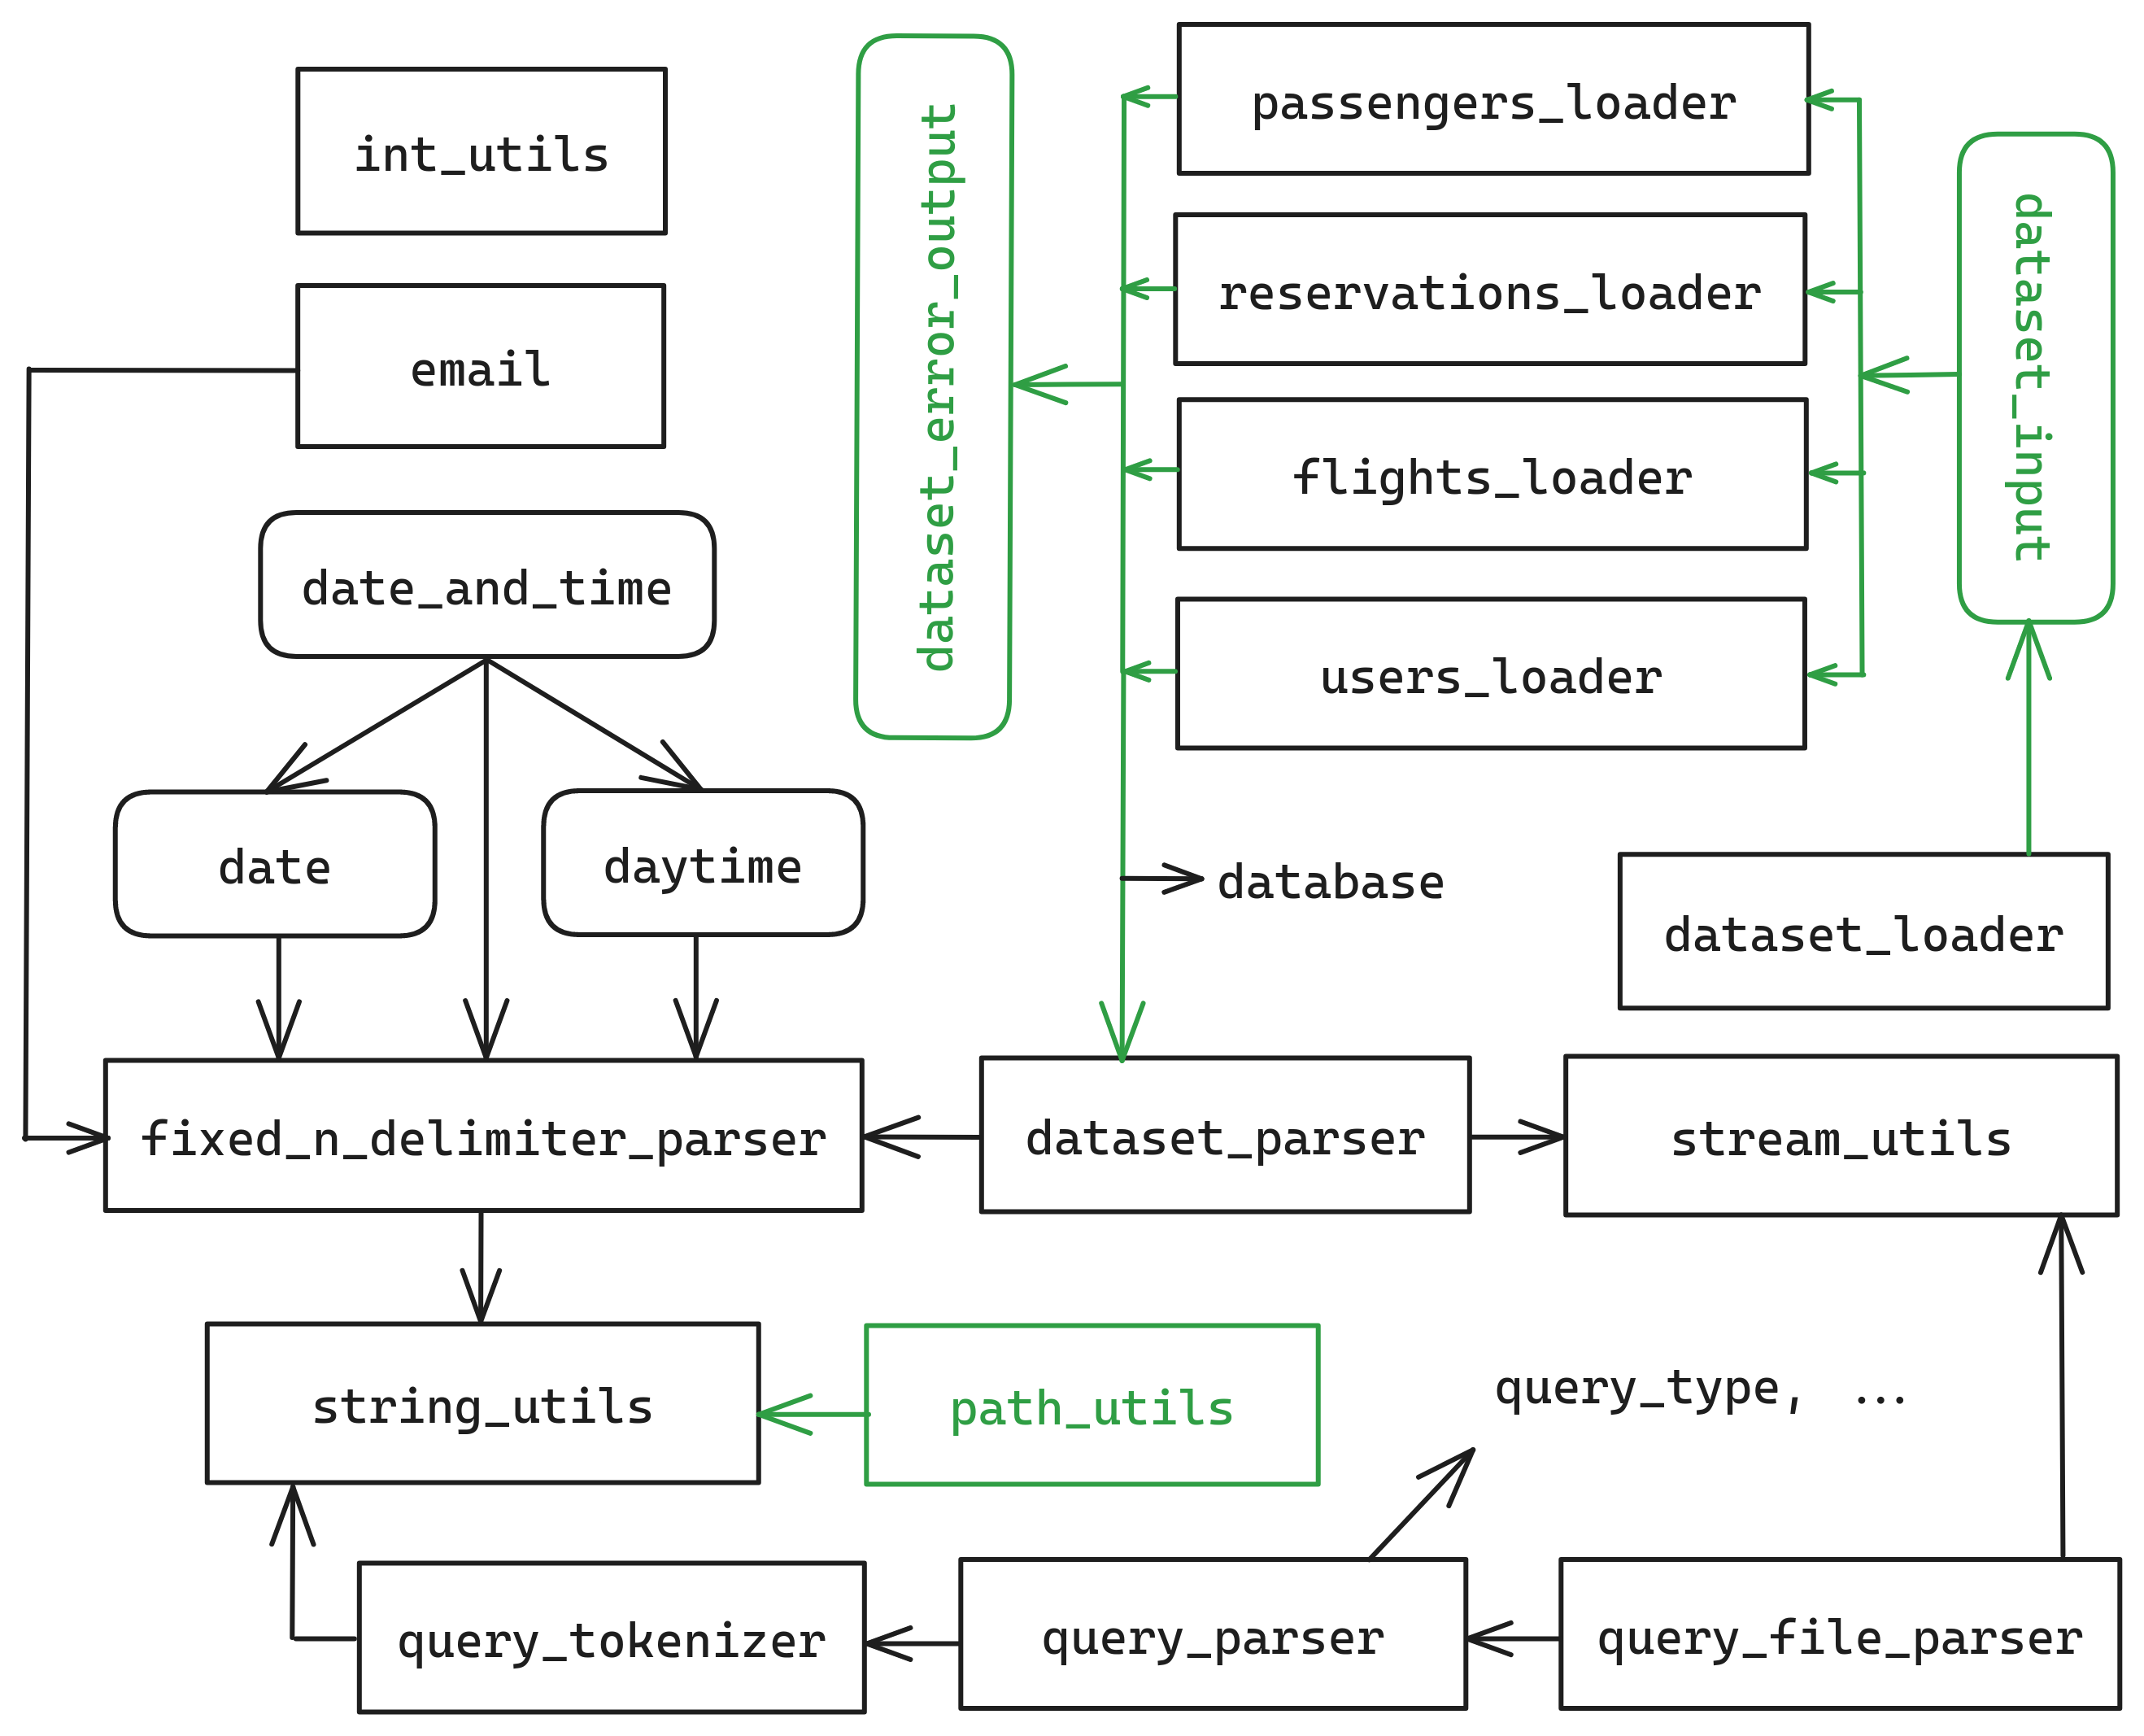
\includegraphics[scale=0.17]{res-fase2/parsing.png}
    \caption{Diagrama de dependências do subsistema de \emph{parsing}}
    \label{fig:parsing}
\end{figure}

Nesta fase do projeto, separámos em diferentes módulos as funcionalidades de \emph{input} de dados
e \emph{output} de erros num \emph{dataset}, antes concentradas no \texttt{dataset\_loader}. Agora,
este módulo apenas gere duas estruturas de dados formadas por \emph{handles} de ficheiros,
\texttt{dataset\_input} e \texttt{dataset\_error\_output}. Ademais, adicionámos o módulo
\texttt{path\_utils}, para manipulação de caminhos para ficheiros.

\subsection{Entidades}
\label{sec:entities}

\begin{figure}[ht]
    \centering
    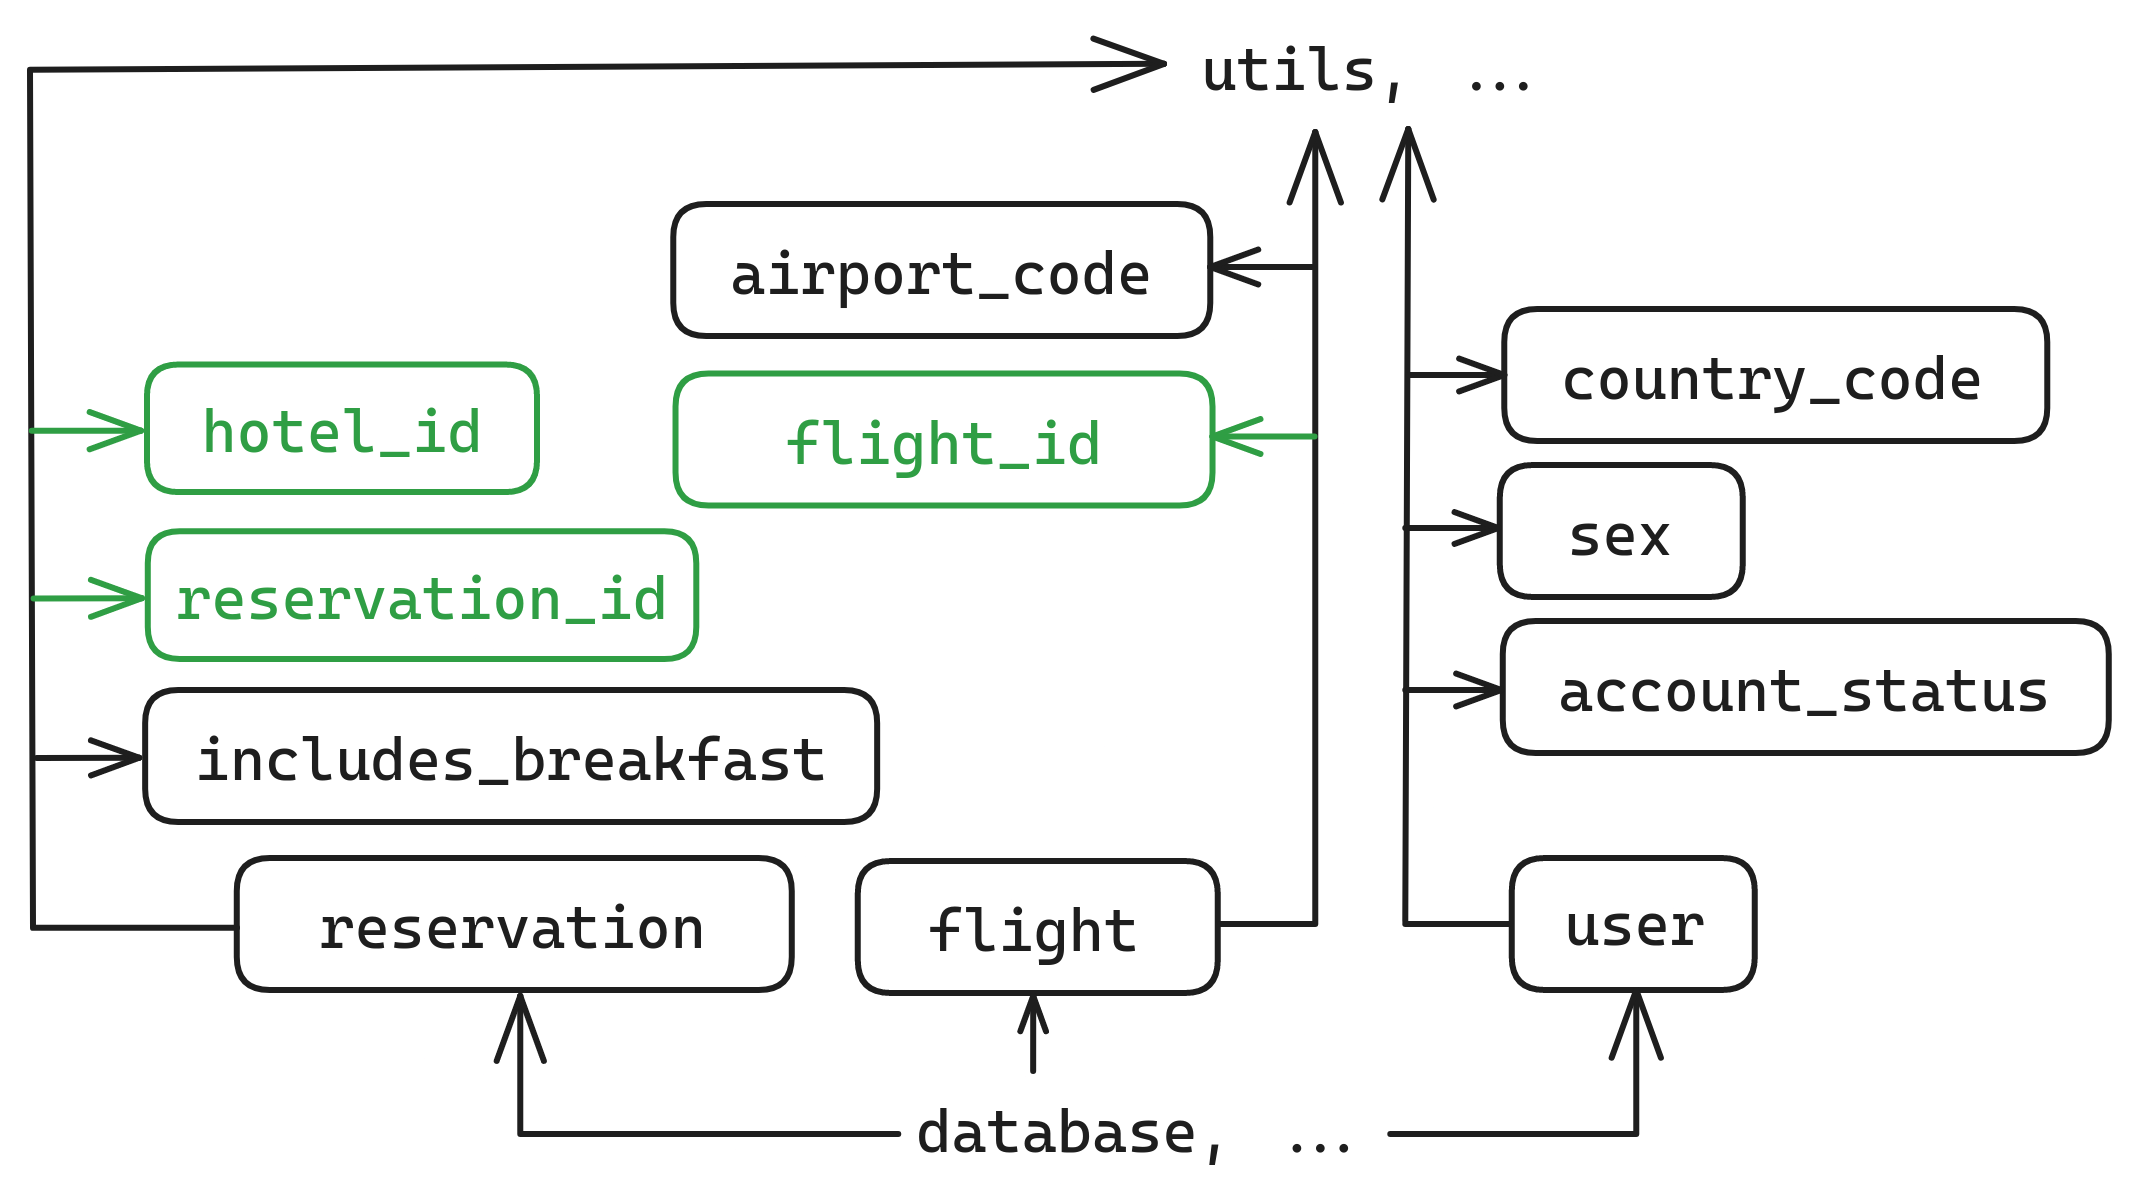
\includegraphics[scale=0.2]{res-fase2/entities.png}
    \caption{Diagrama de dependências das entidades da aplicação}
    \label{fig:entities}
\end{figure}

Nas entidades, criámos módulos para os identificadores de voos, reservas e hotéis. Estes são
armazenados como inteiros, logo exigindo \emph{parsing} e uma forma de serem apresentados
textualmente, código que antes se encontrava em duplicado em vários locais da aplicação. Ademais,
passaram a ser os \emph{setters} das entidades a validar se os valores providenciados para os seus
campos são válidos. Anteriormente, este era o trabalho dos módulos \texttt{*\_loader}, sendo
possível ao programador, usando \emph{setters}, criar uma entidade inválida.

\subsection{Catálogos}
\label{sec:catalogs}

\begin{figure}[ht]
    \centering
    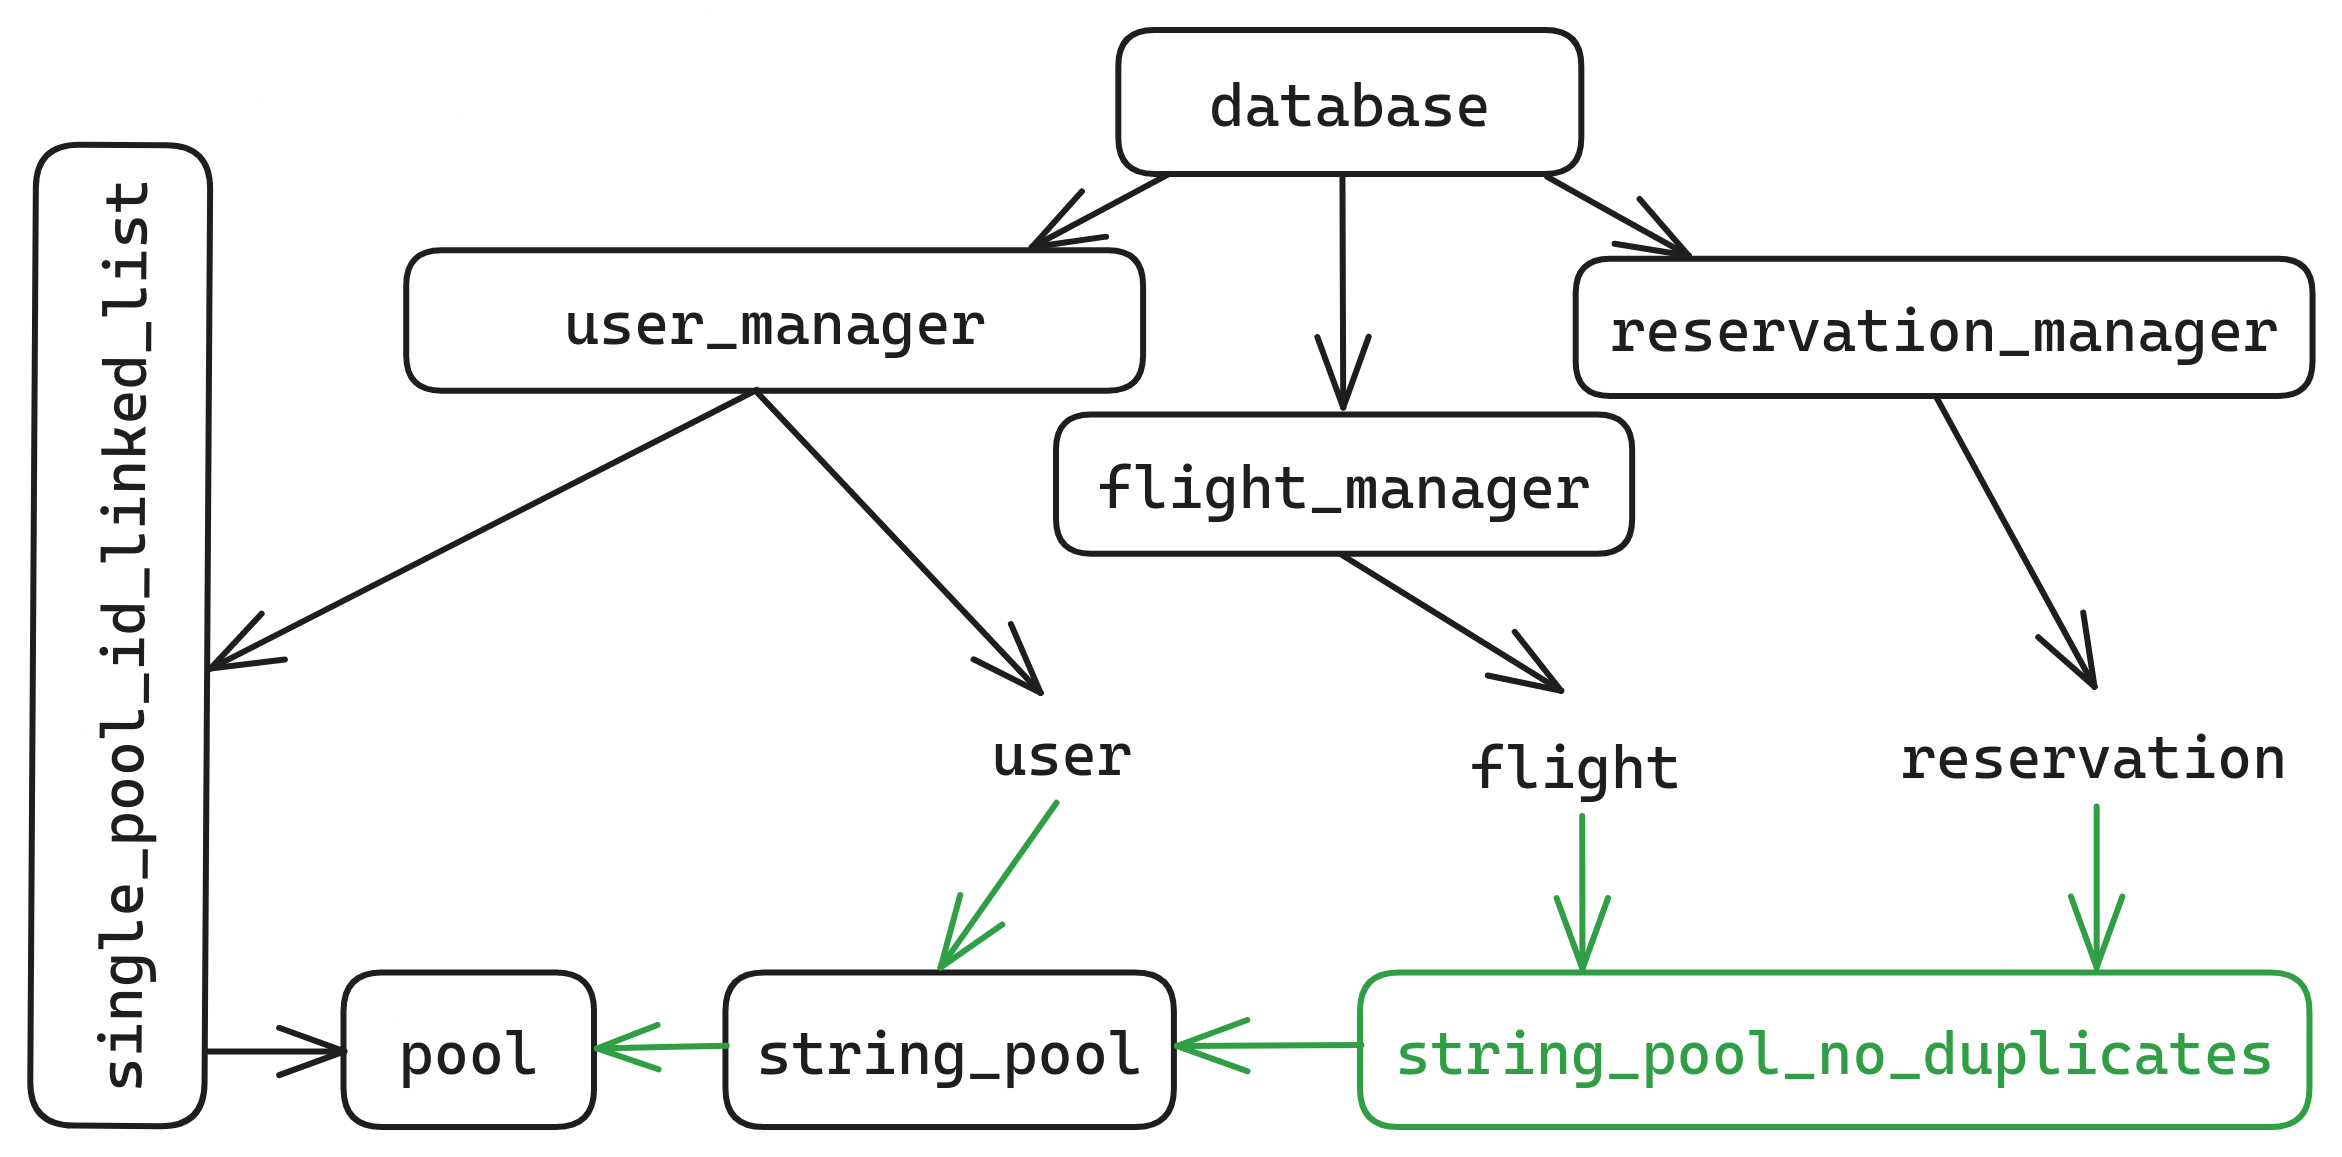
\includegraphics[scale=0.17]{res-fase2/database.png}
    \caption{Diagrama de dependências dos catálogos na aplicação}
    \label{fig:catalogs}
\end{figure}

De modo a diminuir o uso de memória da aplicação, criámos o \texttt{string\_pool\_no\_duplicates},
um novo alocador que armazena apenas uma vez \emph{strings} sujeitas a repetição, como nomes de
hotéis e de companhias aéreas.

Quanto às novas relações de dependência, removemos muito código duplicado ao adaptar a
\texttt{pool}, para com ela ser possível implementar a \texttt{string\_pool}. Ademais, as entidades
passam a depender dos alocadores, por motivos explicados em
\nameref{sec:allocator-conciliation}.

\subsection{\emph{Queries}}
\label{sec:queries}

\begin{figure}[ht]
    \centering
    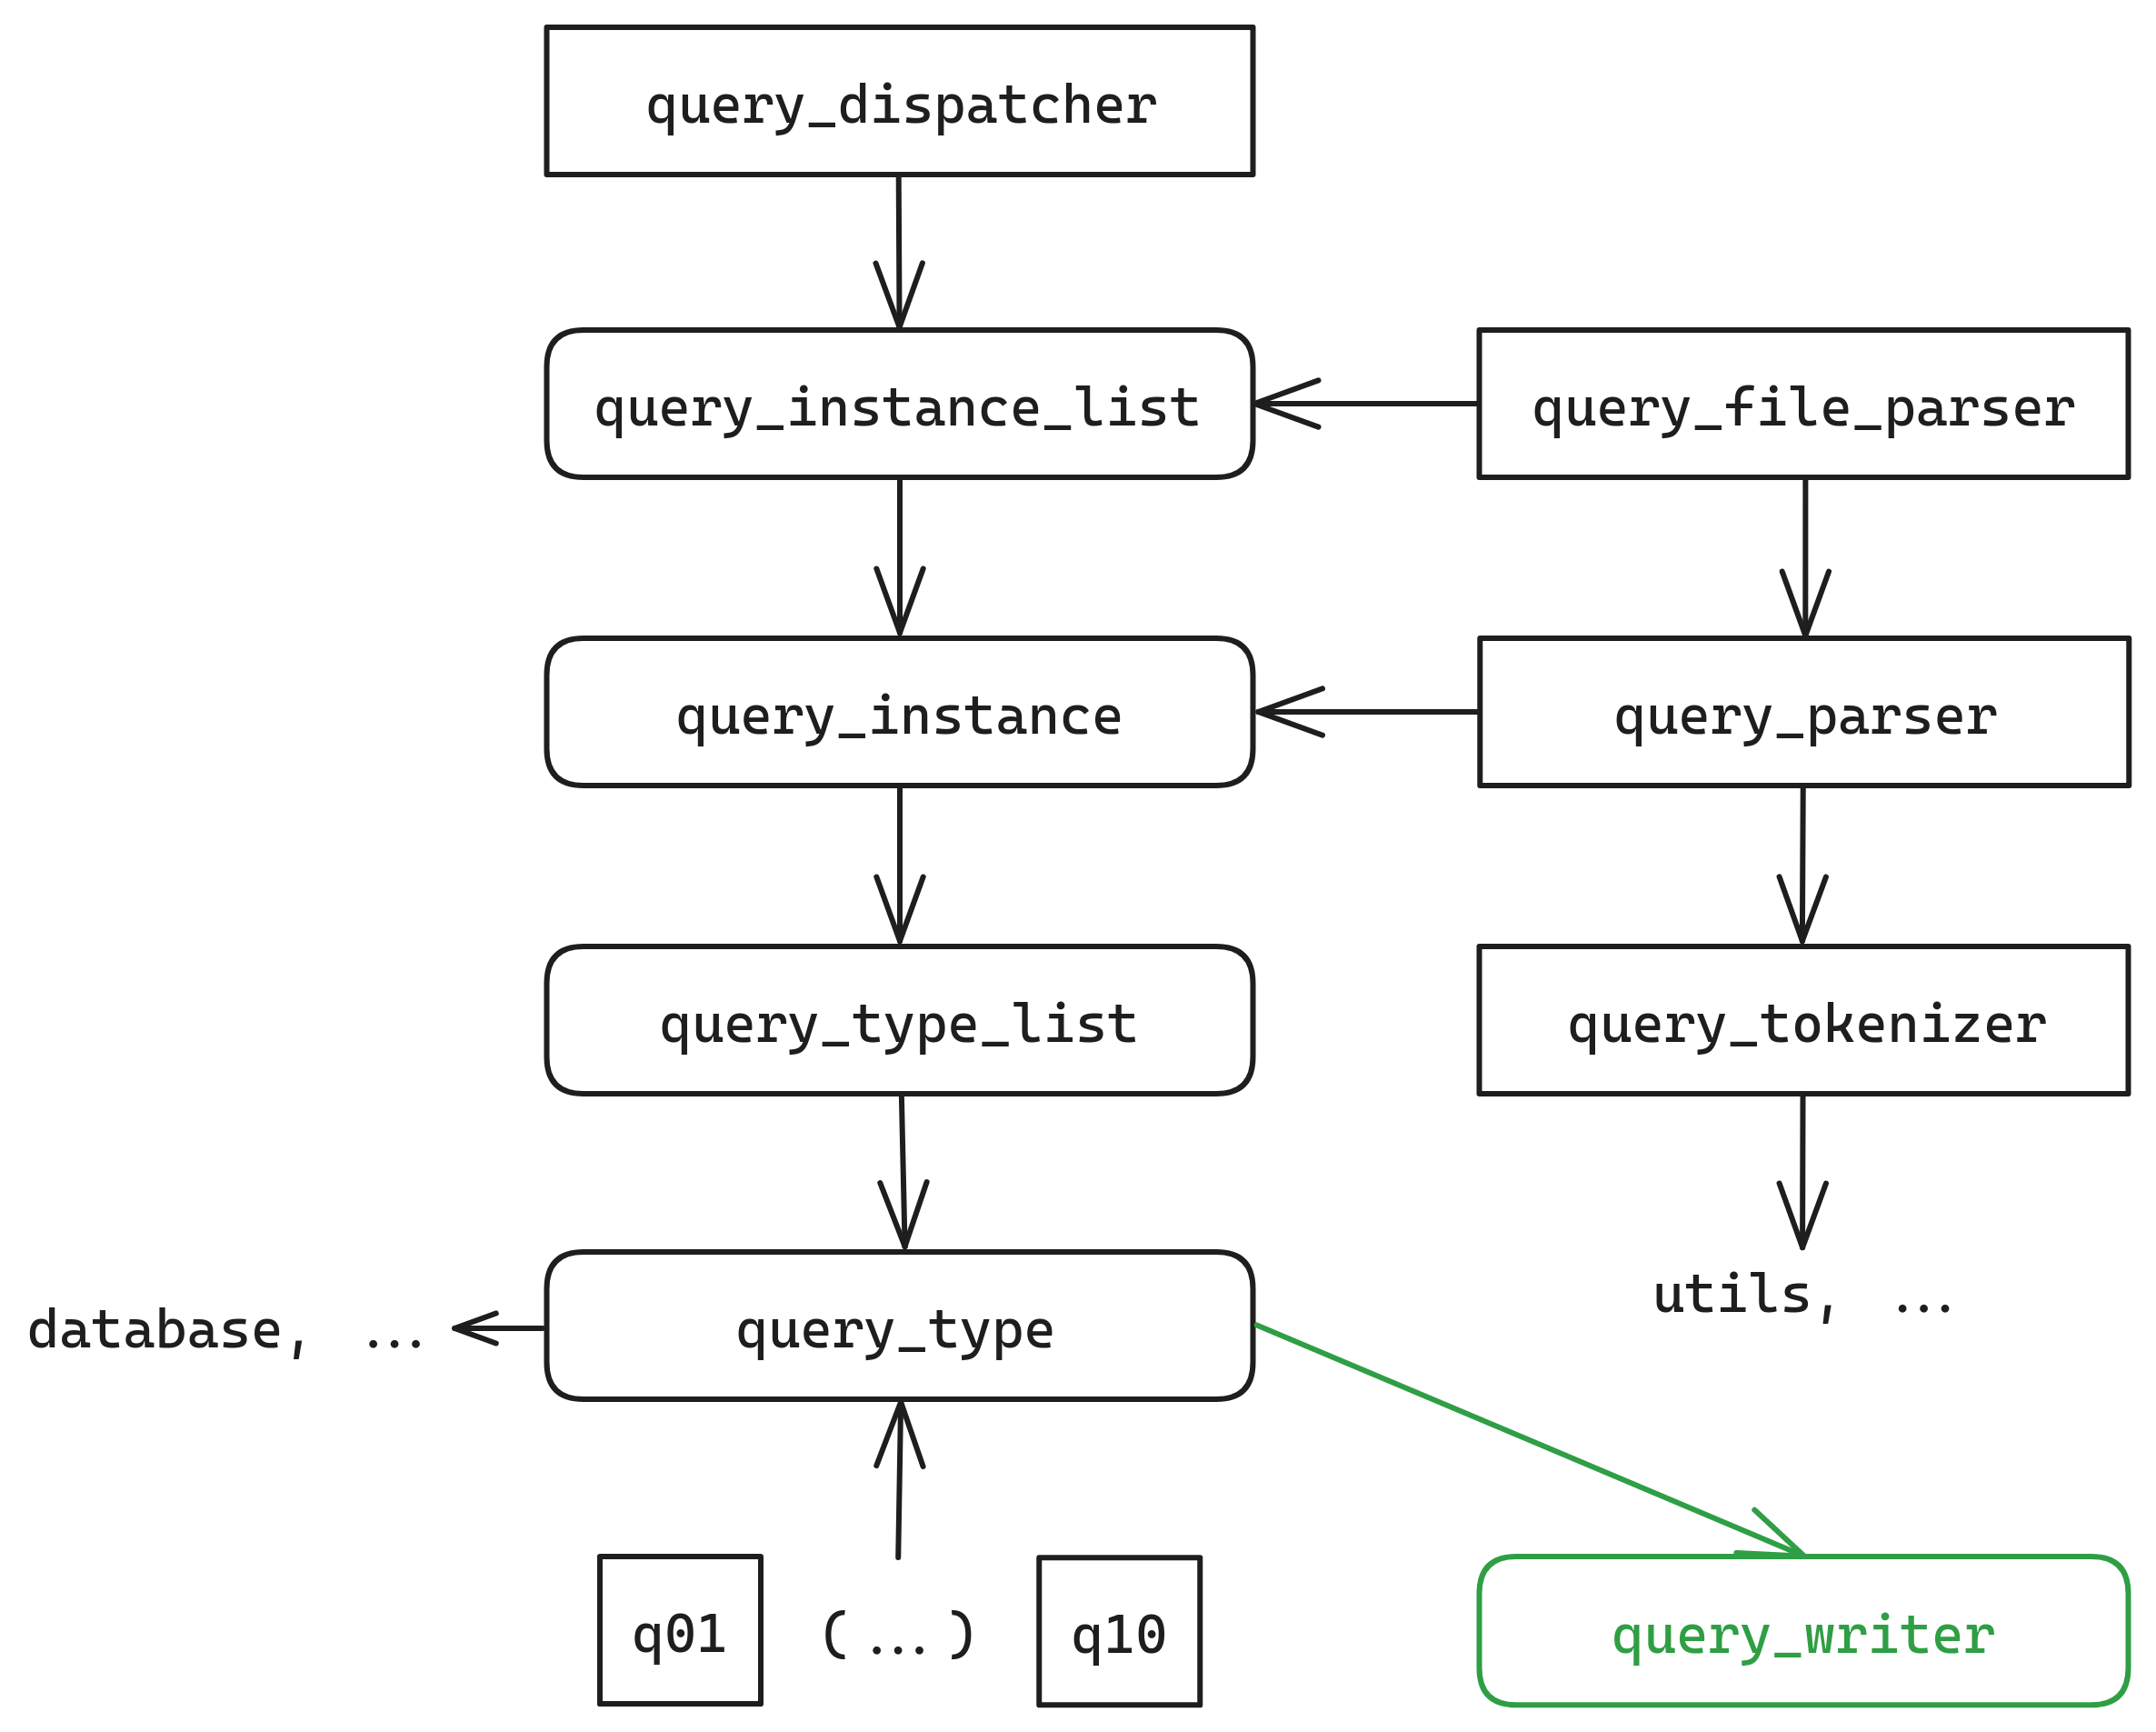
\includegraphics[scale=0.17]{res-fase2/queries.png}
    \caption{Diagrama de dependências do subsistema de \emph{queries}}
    \label{fig:queries}
\end{figure}

Como todas as \emph{queries} apresentam a mesma formatação de \emph{output}, adicionámos a estrutura
\texttt{query\_writer}, que formata o \emph{output} de uma \emph{query} automaticamente, e o
escreve para um ficheiro (modo \emph{batch}) ou para um conjunto de linhas em memória (modo
interativo). Segue-se a descrição do funcionamento das \emph{queries} novas e das que sofreram
mudanças significativas:

\begin{itemize}
    \item \textbf{Q05} - Listagem dos voos com origem num dado aeroporto entre duas datas. Com uma
                         única iteração pelos voos para todas as \emph{queries} deste tipo,
                         verifica-se se cada voo cumpre as condições para ser parte da resposta
                         a uma \emph{query}. Em caso afirmativo, adiciona-se esse voo a um
                         \emph{array}, associado à \emph{query} através de uma tabela de
                         \emph{hash}. A execução de cada \emph{query} passa apenas pela ordenação e
                         apresentação do seu \emph{array} correspondente.

    \item \textbf{Q07} - Listagem dos aeroportos com maior mediana de atrasos. Com uma única
                         iteração pelos voos para todas as \emph{queries} deste tipo, gera-se uma
                         tabela de \emph{hash} que associa aeroportos a \emph{arrays} de atrasos.
                         Depois, calcula-se a mediana para cada \emph{array} (ordenação seguida do
                         ponto médio), gerando-se outra tabela de \emph{hash}, entre aeroportos e
                         medianas de atrasos. Executar cada \emph{query} consiste na consulta direta
                         desta tabela.

    \item \textbf{Q08} - Cálculo da receita de um hotel entre duas datas. Com uma única iteração
                         pelas reservas para todas as \emph{queries} deste tipo, gera-se uma tabela
                         de \emph{hash} que associa pares hotel + intervalo de datas às suas
                         receitas. Interseta-se, para cada reserva, o intervalo de noites dormidas
                         com o pedido na \emph{query}, para o cálculo do número de noites e da
                         receita total. Executar cada \emph{query} consiste simplesmente na consulta
                         da tabela gerada.

    \item \textbf{Q09} - Listagem de todos os utilizadores cujo nome comece com um dado prefixo. A
                         nova implementação desta \emph{query} é muito semelhante à da \textbf{Q05},
                         mas iterando pelos utilizadores em vez dos voos. Esta solução é
                         significativamente mais veloz que a anterior, que fazia uma iteração pelos
                         utilizadores por \emph{query}. Considerámos a possibilidade
                         de gerar um índice de pesquisa usando \emph{tries}, mas optámos por não
                         tornar o nosso código muito complexo para otimizar algo responsável por uma
                         fração mínima do tempo total do programa.

    \item \textbf{Q10} - {\color{red}Ainda tenho de otimizar isto}
\end{itemize}

\subsection{Modo interativo}
\label{sec:interactive-mode}

\begin{figure}[ht]
    \centering
    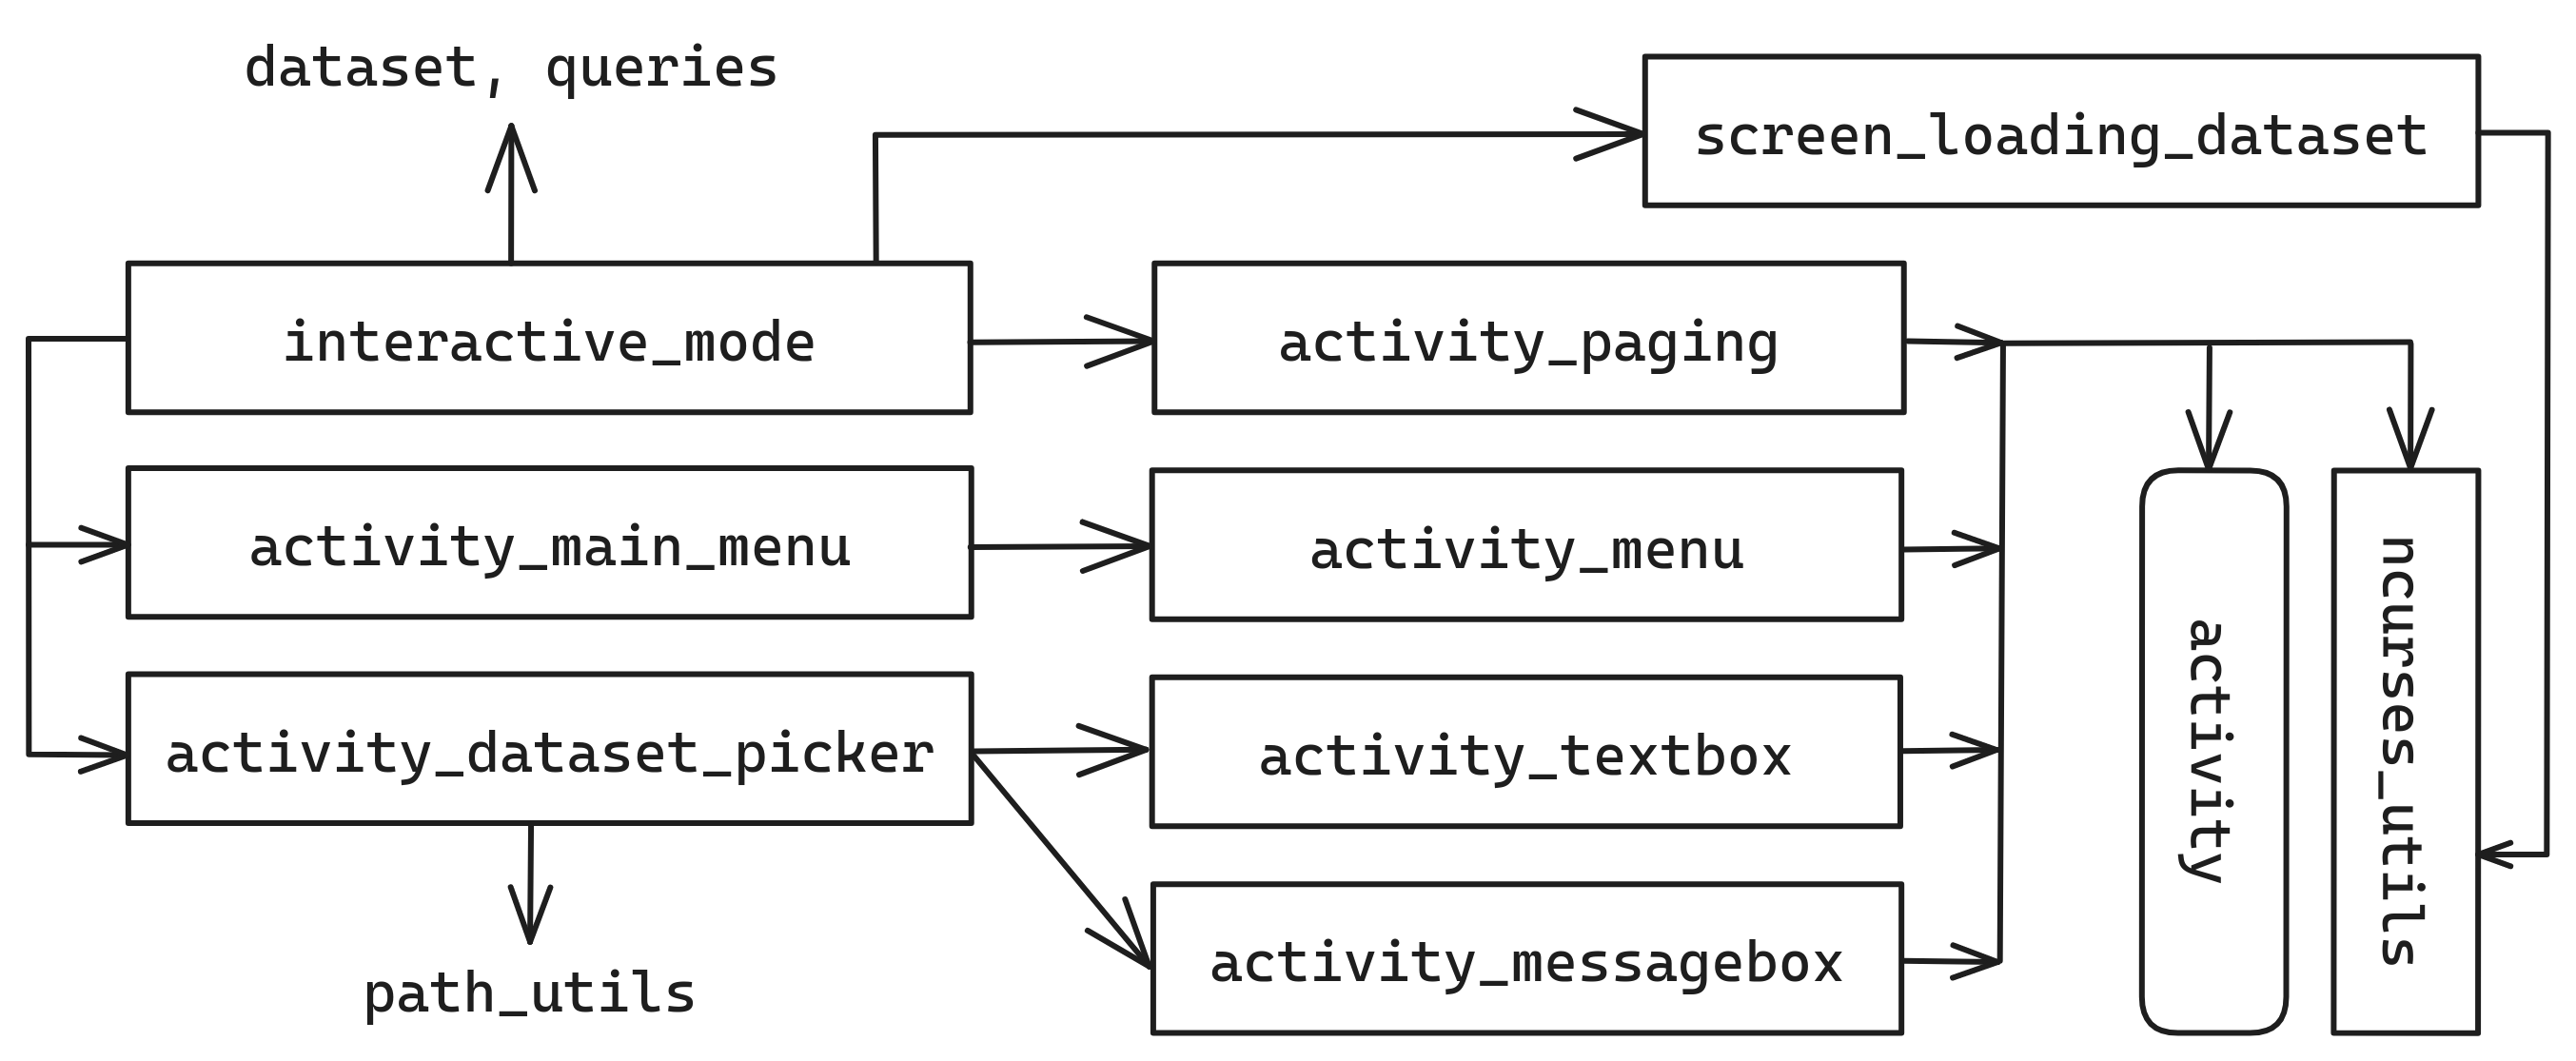
\includegraphics[scale=0.17]{res-fase2/interactive.png}
    \caption{Diagrama de dependências do modo interativo}
    \label{fig:interactive}
\end{figure}

O modo interativo revolve à volta do conceito de atividade (\texttt{activity}), que gere o
\emph{loop} de eventos de uma interface \texttt{curses}, chamando os \emph{callbacks} com os quais
é definida para responder a esses eventos. Imagens das atividades implementadas podem ser
encontradas em \nameref{sec:interactive-screenshots}. \texttt{screen\_loading\_dataset} não responde
a eventos, mas desenha no ecrã que a aplicação se encontra a ler um \emph{dataset}. O módulo
\texttt{interactive\_mode} é responsável por controlar a troca entre atividades, formando a
aplicação final.

Para maior facilidade de uso, incluímos instruções em todas as interfaces, e desenvolvemos um
navegador de ficheiros para o utilizador não ter de digitar o caminho para um \emph{dataset}.
Ademais, temos excelente suporte para Unicode, que tem em conta que diferentes caracteres podem ter
diferentes dimensões (para o \emph{layout} de interfaces).

\subsection{Subsistema de testes}
\label{sec:testing-subsystem}

\begin{figure}[ht]
    \centering
    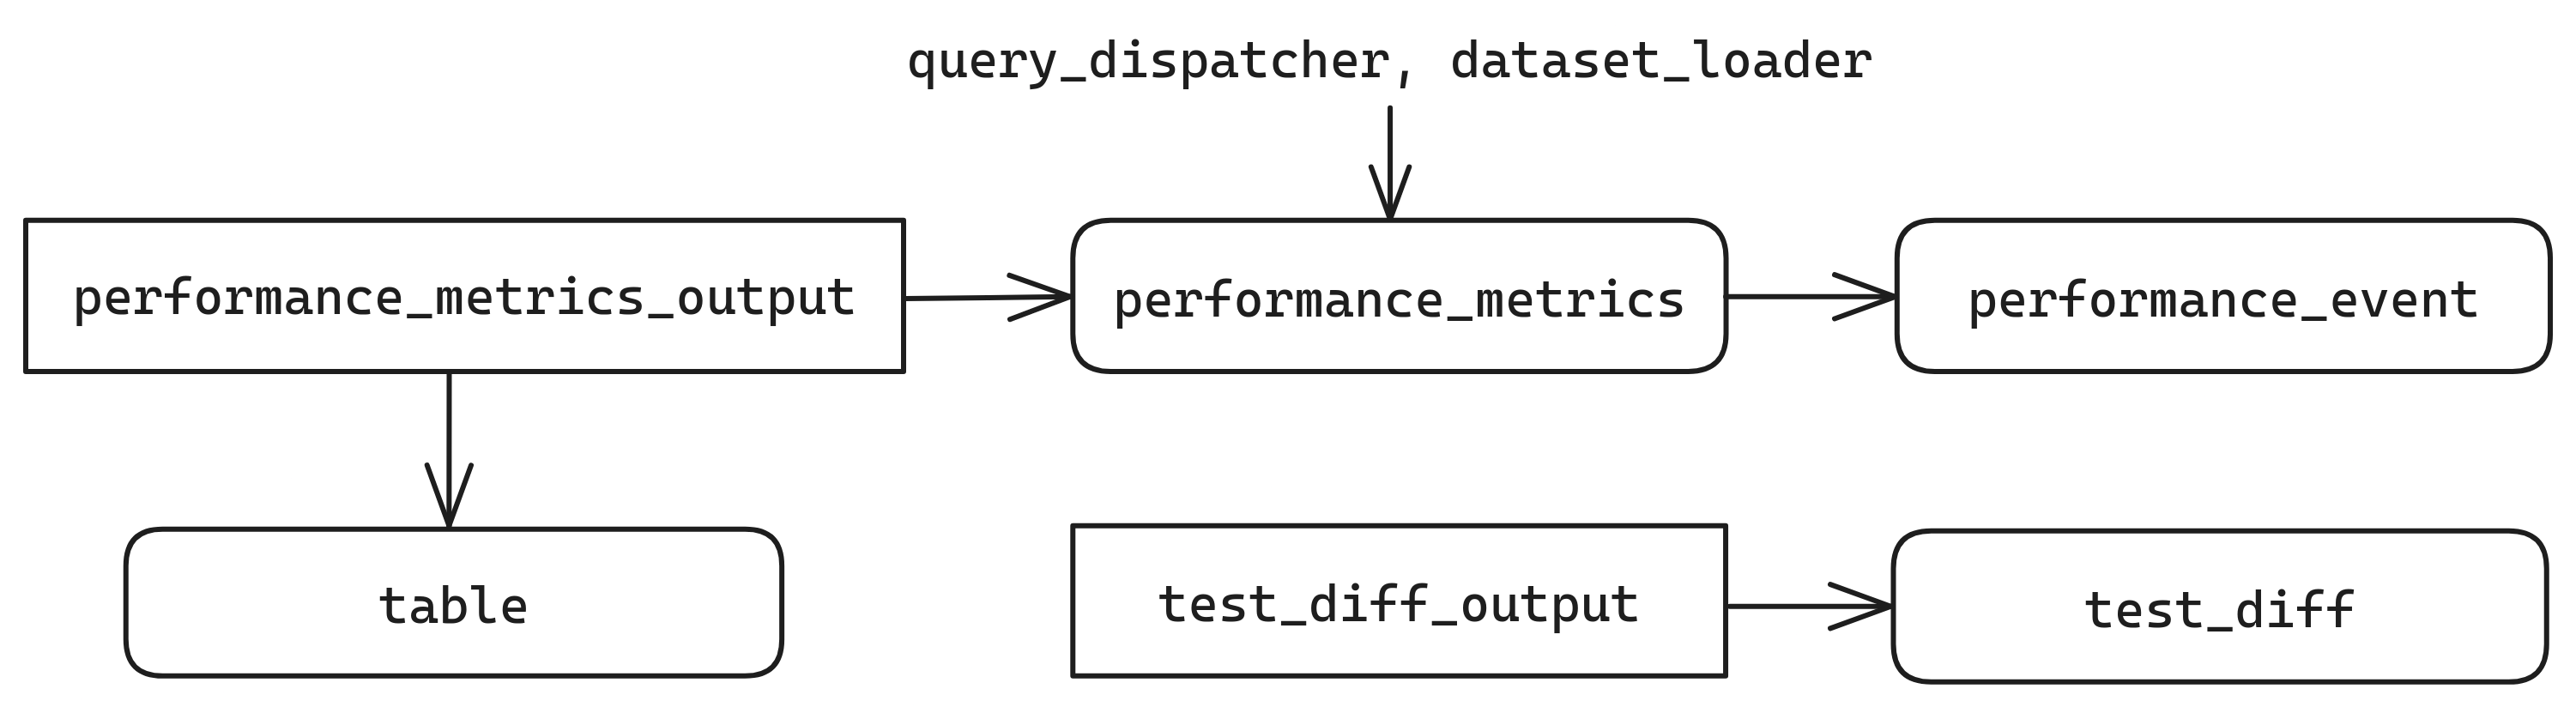
\includegraphics[scale=0.15]{res-fase2/testing.png}
    \caption{Diagrama de dependências do subsistema de testes}
    \label{fig:testing}
\end{figure}

Os testes de desempenho baseiam-se num \texttt{performance\_event}, uma medição do tempo e da
diferença do uso de memória entre dois instantes. \texttt{performance\_metrics} são um conjunto de
eventos de desempenho, produzidos ao longo do decorrer da aplicação, e mostrados ao utilizador no
final da sua execução (\texttt{performance\_metrics\_output}). Este módulo apresentada várias
tabelas (\texttt{table}), relativas ao uso de recursos computacionais na leitura de cada parte do
\emph{dataset} e na execução de cada \emph{query} (tempo individual, estatístico e amortizado).

Os testes funcionais são implementados por \texttt{test\_diff}, que calcula as diferenças entre
duas diretorias (ficheiros em falta, em excesso, e diferenças entre ficheiros), que são depois
apresentadas ao utilizador por \texttt{test\_diff\_output}. Imagens dos resultados de ambos os tipos
de teste encontram-se em \nameref{sec:testing-screenshots}.

\section{Modularidade e encapsulamento}
\label{sec:modularity-and-encapsulation}

\subsection{Modularidade}
\label{sec:modularity}

No relatório da primeira fase, afirmámos estar satisfeitos com o nível de modularidade conseguido.
No entanto, tínhamos noção de que havia alguns aspetos a melhorar: separar os módulos de I/O e os
identificadores das entidades. Não só corrigimos estes problemas, como planeámos as novas partes da
aplicação tendo em conta as anteriores falhas na estrutura do programa.

\subsection{Encapsulamento}
\label{sec:encapsulation}

\subsubsection{\emph{The great refactoring}}
\label{sec:the-great-refactoring}

Apesar de, na primeira fase deste trabalho, termos definido \emph{getters} e \emph{setters} para as
estruturas de dados, estávamos cientes da ausência de encapsulamento, pois vários \emph{getters}
devolviam apontadores mutáveis para dados no interior das estruturas. Como nunca escrevíamos para
estes apontadores, torná-los constantes provou-se a melhor solução para o encapsulamento.

Este processo de aplicar a \emph{keyword const} aos argumentos dos métodos e aos seus valores
devolvidos provou-se moroso: a cada \emph{const} adicionado, vários módulos deixavam de compilar
devido a erros de tipos, causando uma reação em cadeia de mudanças necessárias. No processo de
encapsulamento, adicionámos também métodos de cópia profunda (semelhantes aos \emph{copy
constructors} de C++) à maioria das estruturas de dados da aplicação. \footnote{Com exceção de
alocadores (\emph{pools}) e estruturas que contêm \texttt{FILE *}.}

Apercebemo-nos da importância de uma interface modular bem pensada que dispensa mudanças, já que
estas se provaram muito trabalhosas. No modo interativo e no subsistema de testes, como pensámos nas
interfaces dos módulos com encapsulamento em mente, não precisámos de gastar tempo na sua correção.

\subsubsection{Conciliação com alocadores}
\label{sec:allocator-conciliation}

As únicas estruturas de dados que expõem memória do seu interior são os alocadores \texttt{pool} e
\texttt{string\_pool}. Não encaramos isto como um problema no encapsulamento, pois é algo que
qualquer alocador tem de fazer (por exemplo, o método \texttt{malloc} expõe memória da arena com
que é implementado).

Previamente, durante uma inserção na base de dados, as entidades e os seus campos eram alocados
pelos \emph{managers} nas \emph{pools}, e não pelas entidades em si. Resolvemos este problema no
encapsulamento usando uma estratégia semelhante à utilizada na linguagem Zig: se um método precisa
de alocar memória na \emph{heap}, então leva um alocador como argumento:

\begin{center}
    \texttt{fn validate(allocator: Allocator, s: []const u8) Allocator.Error!bool}
\end{center}

Este método de Zig valida texto JSON, levando também como argumento um alocador. Na nossa aplicação
C, é dada a possibilidade de se usar uma \emph{pool}, ou de se passar o valor \texttt{NULL} ao
argumento do alocador, para o uso de \texttt{malloc}:

\begin{center}
    \begin{tabular}{rl}
        \texttt{user\_t *user\_clone(}&\hspace{-3mm}\texttt{pool\_t *allocator,} \\
        &\hspace{-3mm}\texttt{string\_pool\_t *string\_allocator,} \\
        &\hspace{-3mm}\texttt{const user\_t *user);}
    \end{tabular}
\end{center}

\subsubsection{Conciliação com a \texttt{glib}}
\label{sec:glib-conciliation}

O uso de \emph{const} é um contrato de que um módulo não irá modificar um objeto. A documentação das
estruturas genéricas da \texttt{glib} assegura isto.\footnote{Há algumas exceções (como uma função
\texttt{GDestroyNotify} ser providenciada), mas garantimos que a nossa solução para este problema
não permite nenhuma destas.} No entanto, estas utilizam \texttt{void *} sem \texttt{const}, dado
que os programadores podem querer utilizá-las para armazenar dados não constantes.

Para podermos usar a \texttt{glib} para armazenar apontadores constantes, criámos \emph{wrappers}
que os aceitam e lhes tiram o \emph{modifier const} antes de interagirem com uma estrutura da
\texttt{glib}, algo que podemos que podemos fazer com o aval da documentação. Estes \emph{wrappers}
são preferíveis a usar as estruturas da \texttt{glib} diretamente e fazer \emph{casts} quando
necessário, pois reduzimos o potencial de erro do programador a pequenos excertos de código, em
vez de toda a aplicação, de um modo semelhante a conceito de \texttt{unsafe} em Rust.

\section{Desempenho}
\label{sec:performance}

\subsection{Melhorias}
\label{sec:performance-improvements}

Apesar do desempenho excelente que a nossa aplicação apresentou quando os \emph{datasets} de maior
dimensão foram adicionados à plataforma de testes, procurámos mesmo assim continuar a otimizar o
nosso programa.

Para reduzir ainda mais o uso de memória, introduzimos a \texttt{string\_pool\_no\_duplicates}, que
evita armazenar \emph{strings} repetidas. Ademais, reordenamos os campos nas estruturas de dados das
entidades, de modo a reduzir o \emph{padding} e o número de \emph{bytes} ocupados por cada uma.

A maioria do tempo de execução é gasto no \emph{parsing} do \emph{dataset}, onde apenas conseguimos
alcançar micro-otimizações nos métodos mais chamados, determinados com recurso ao
\texttt{callgrind}. A única melhoria significativa que obtivemos resultou da substituição do
\texttt{strsep} por um novo método, que considera apenas um delimitador.

Ademais, como a execução das \emph{queries} já era muito veloz, o nosso foco foi o de simplificar
o código, e não o de o otimizar com melhores estruturas de dados. Várias vezes as estruturas simples
se provaram mais rápidas do que outras mais complexas, uma lembrança de que a complexidade
algorítmica é assintótica. Foi importante garantir que os catálogos usavam as
melhores estruturas para acelerar as \emph{queries}, mas tal não se provou tão relevante para dados
auxiliares usados durante a execução das mesmas.

\subsection{\emph{Benchmarking}}
\label{sec:benchmarking}

Para testar o desempenho do programa, corremos, nos seguintes sistemas, 500 \emph{queries} no
\emph{dataset} grande com erros:

\begin{center}
    \begin{tabular}{|l|c|c|c|c|}
        \hline
        & Desktop & Laptop & Mac & Tablet \\
        \hline
        CPU & Intel i3-7100 & Ryzen & M1 & Mediatek Helio P22T \\
        \hline
        Frequência\footnote{Em sistemas heterogéneos, a frequência do \emph{cluster} de maior
                            desempenho, dado que o nosso programa apenas usa um núcleo.} &
        3.9 GHz & ? & ? & 2.3 GHz \\
        \hline
        Memória & DDR4 2400 MT/s & ? & ? & LPDDR4X 4266 MT/s \\
        \hline
        Linux & 6.6.11 (chroot) & ? & ? & ? \\
        \hline
        Compilador & gcc 12.2.0 & ? & ? & ? \\
        \hline
    \end{tabular}
\end{center}

A aplicação foi executada 10 vezes, com as execuções mais rápida e a mais lenta removidas. A partir
das 8 restantes, calculam-se as seguintes médias de tempo, em segundos:

\begin{center}
    \begin{tabular}{|l|c|c|c|c|}
        \hline
        & Desktop & Laptop & Mac & Tablet \\
        \hline
        Utilizadores & ? & ? & ? & ? \\
        \hline
        Voos & ? & ? & ? & ? \\
        \hline
        Reservas & ? & ? & ? & ? \\
        \hline
        Passageiros & ? & ? & ? & ? \\
        \hline
        Q10 & ? & ? & ? & ? \\
        \hline
        Restantes \emph{queries} & ? & ? & ? & ? \\
        \hline
        Total & ? & ? & ? & ? \\
        \hline
    \end{tabular}
\end{center}


% TODO - benchmarking

\subsection{Possíveis melhorias}
\label{sec:possible-performance-improvements}

A parte mais lenta do nosso programa é a leitura de um dataset. Como as estruturas de dados
presentes nos catálogos apresentam tempo de inserção amortizado $\Theta(1)$ e já otimizámos a
localidade de memória o mais que pudemos (alocadores customizados), não vemos mais otimizações que
não sacrifiquem a modularidade e encapsulamento que não a paralelização da leitura do
\emph{dataset}:

\begin{figure}[h]
    \centering
    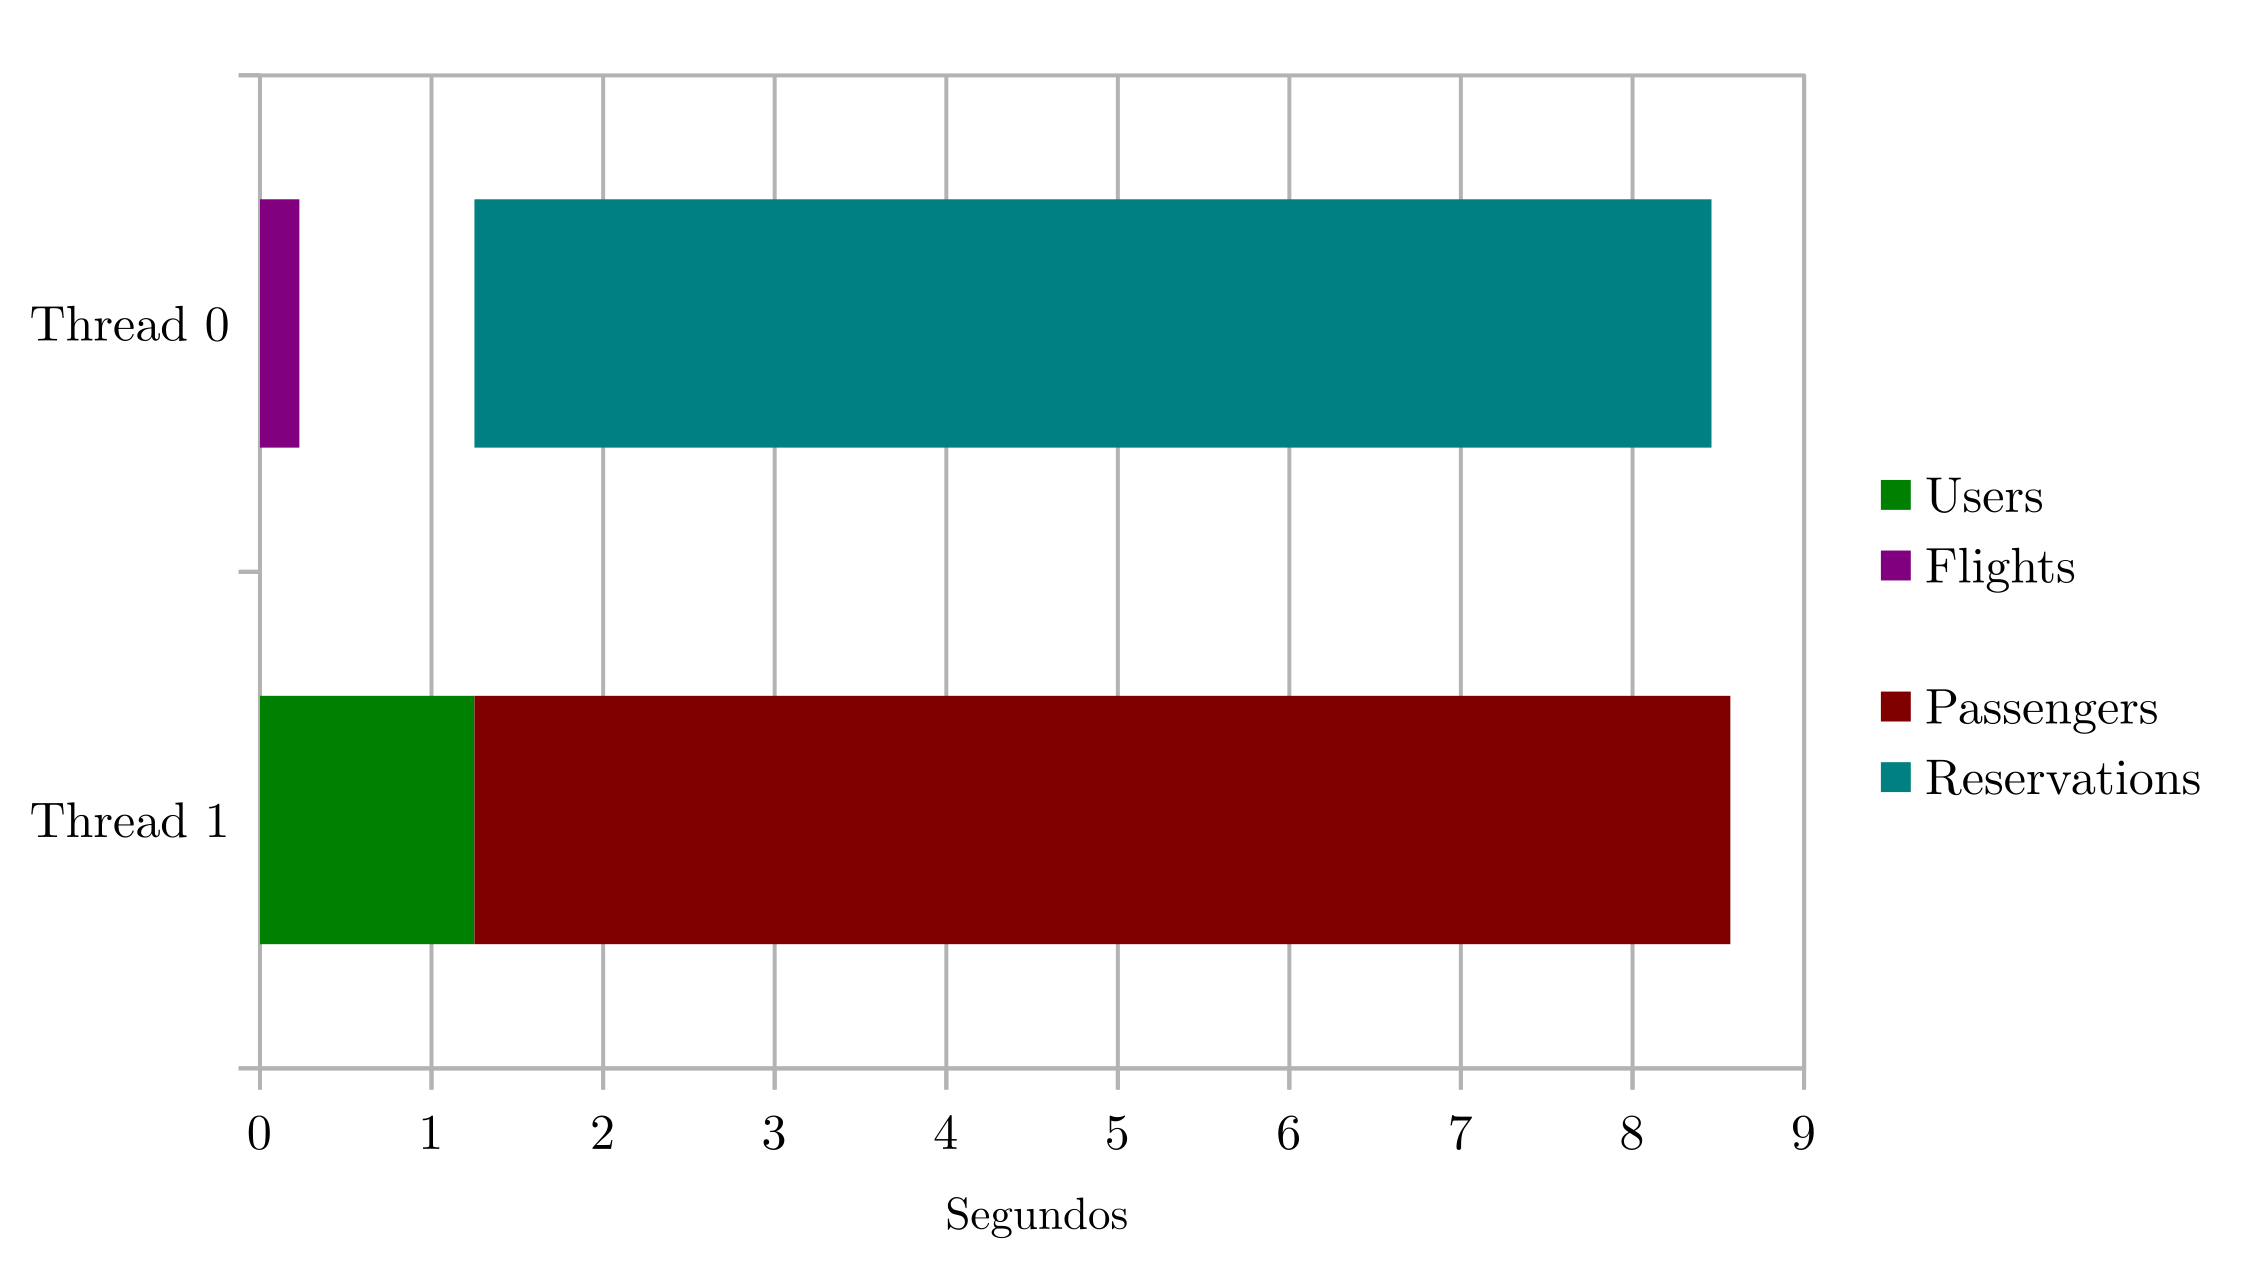
\includegraphics[scale=0.20]{res-fase2/threading.png}
    \caption{Possível distribuição de tarefas por \emph{threads}, com os tempos da
             \hyperref[fig:dataset-screenshot]{Figura \ref*{fig:dataset-screenshot}}}
    \label{fig:threading}
\end{figure}

Usando a distribuição de tarefas acima, que garante a condição das reservas e passageiros serem
lidos após os utilizadores, conseguimos reduzir o tempo de \emph{parsing} de 16 s para um mínimo
teórico 8.6 s! A única dependência de dados que encontrámos, um alocador, é facilmente resolúvel
com o uso de dois alocadores distintos para as relações utilizador -- voo / reserva.

Acreditamos que o desempenho das \emph{query} 10 ainda pode ser melhorado. Quanto às restantes,
não vemos muito interesse na sua otimização, mesmo que possível, dado que constituem uma fração de
tempo muito pequena no modo \emph{batch} e são quase instantâneas para um utilizador do modo
interativo.

\hspace{1cm}\parbox{15cm}{\small
    The real problem is that programmers have spent far too much time worrying about efficiency in
    the wrong places and at the wrong times; premature optimization is the root of all evil (or at
    least most of it) in programming.

    \begin{flushright}
        -- Donald Knuth, Computer Programming as an Art, p. 671
    \end{flushright}
}

\section{Conclusão}
\label{sec:conclusion}

{\color{red} TODO}

\pagebreak
\section{Anexos}
\label{sec:annexes}

\subsection{\emph{Screenshots} do modo interativo}
\label{sec:interactive-screenshots}

\begin{figure}[H]
    \centering
    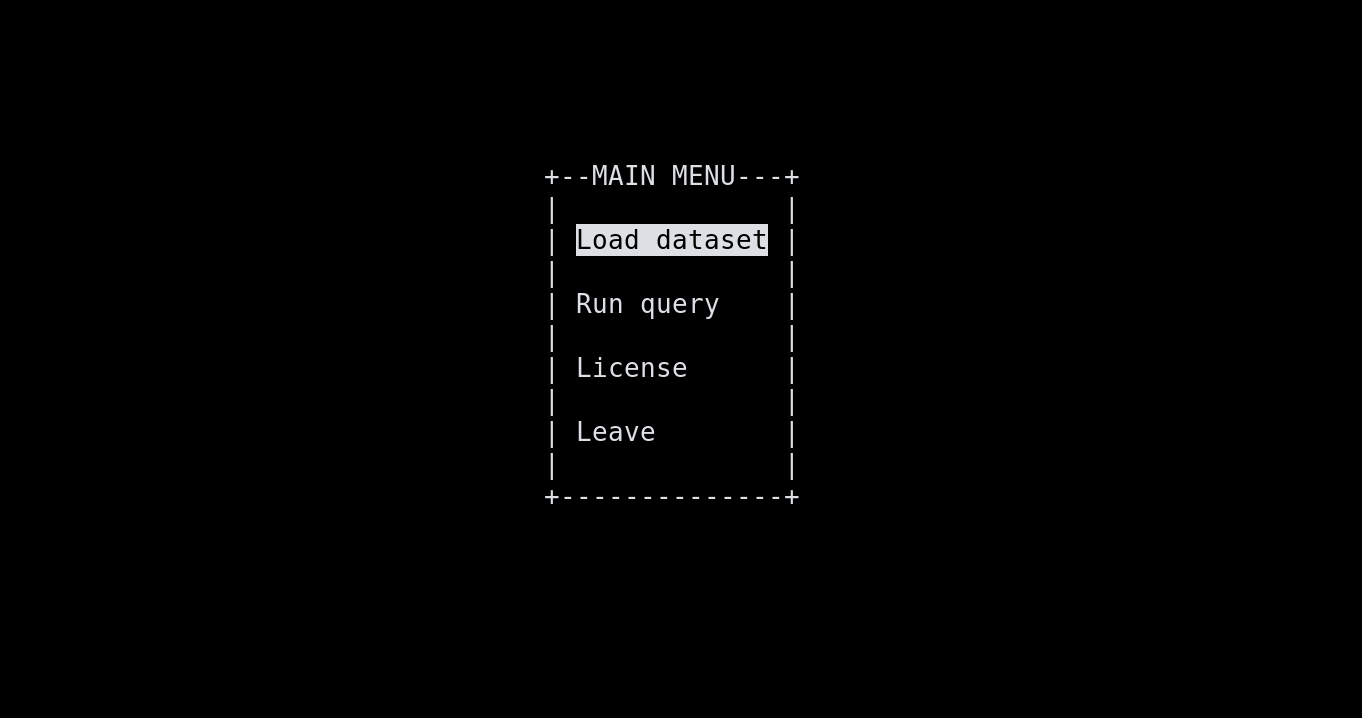
\includegraphics[scale=0.25]{res-fase2/interactive_screenshots/main_menu.png}
    \caption{Menu (\texttt{activity\_menu}), em particular, o menu principal
             (\texttt{activity\_main\_menu})}
    \label{fig:main_menu}
\end{figure}

\begin{figure}[H]
    \centering
    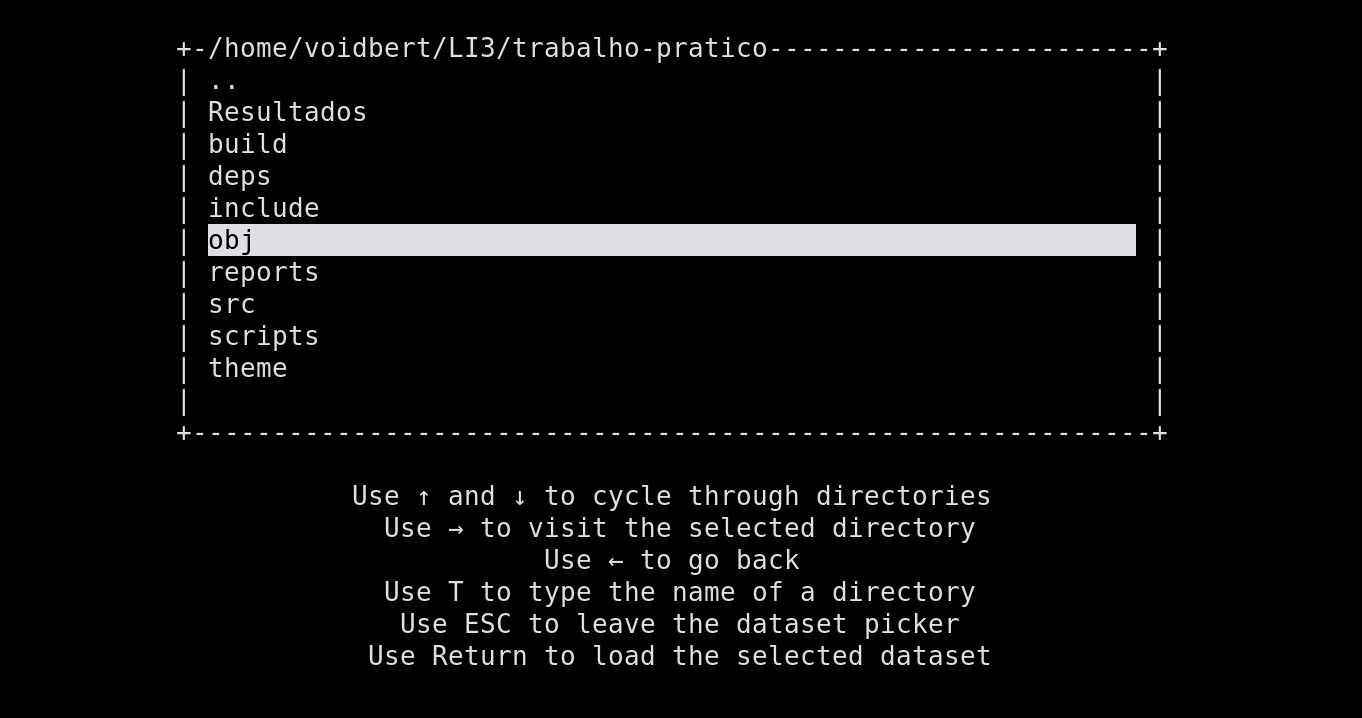
\includegraphics[scale=0.25]{res-fase2/interactive_screenshots/dataset_picker.png}
    \caption{Navegador de ficheiros para a escolha de um \emph{dataset}
             (\texttt{activity\_dataset\_picker})}
    \label{fig:dataset_picker}
\end{figure}

\begin{figure}[H]
    \centering
    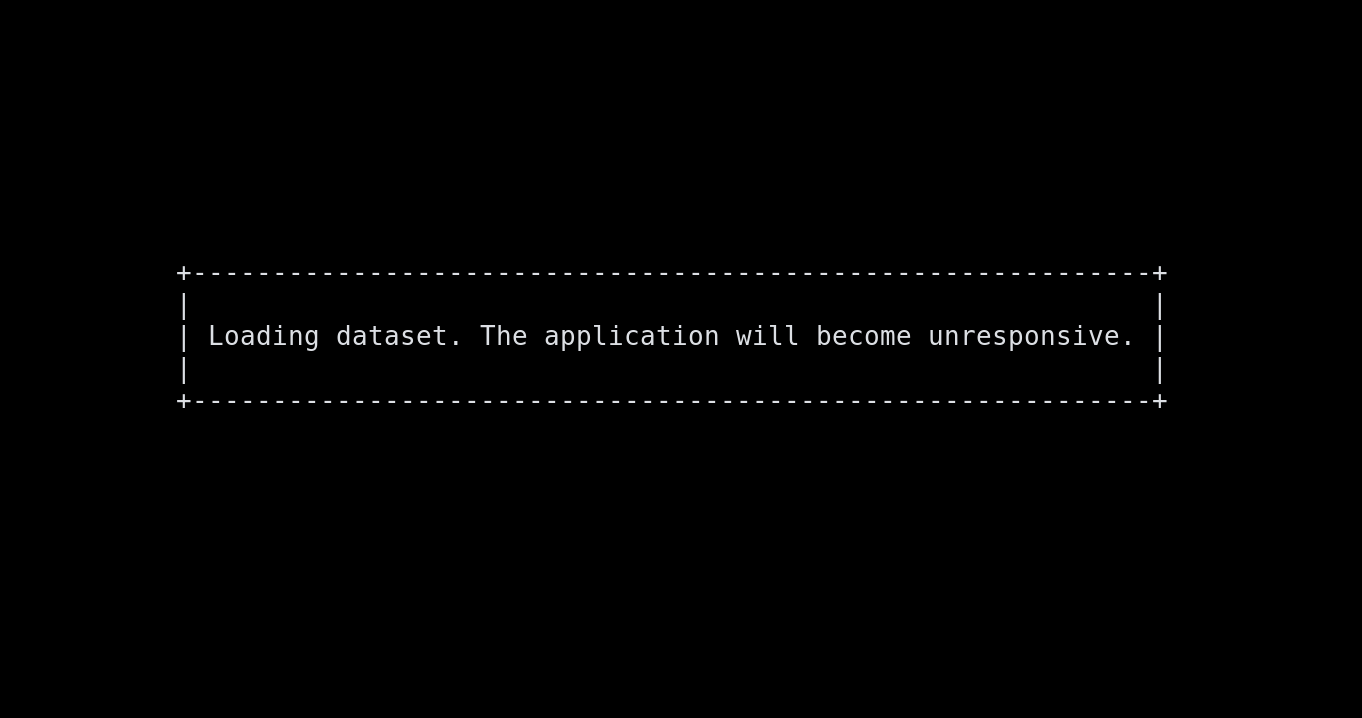
\includegraphics[scale=0.25]{res-fase2/interactive_screenshots/loading_dataset.png}
    \caption{Ecrã durante a leitura de um \emph{dataset} (\texttt{screen\_loading\_dataset})}
    \label{fig:loading_dataset}
\end{figure}

\begin{figure}[H]
    \centering
    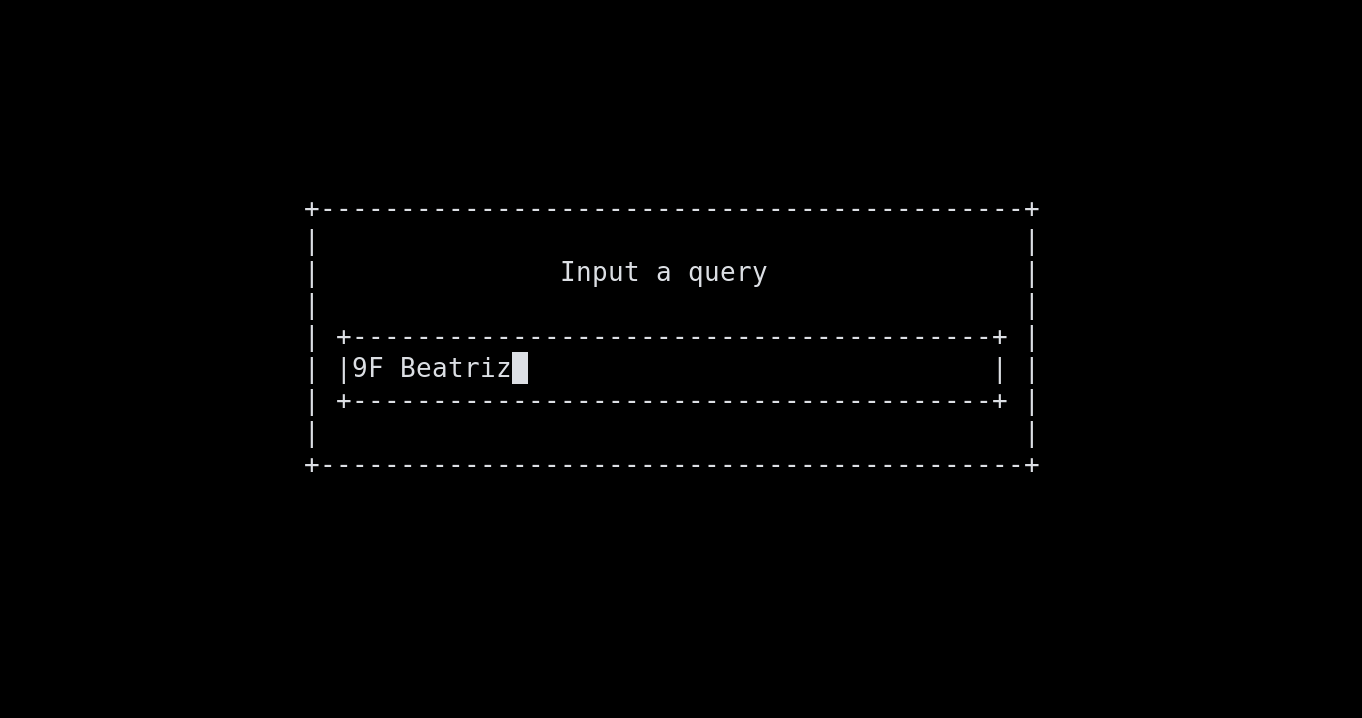
\includegraphics[scale=0.25]{res-fase2/interactive_screenshots/textbox.png}
    \caption{Caixa de texto para a entrada de uma \emph{query} (\texttt{activity\_textbox})}
    \label{fig:textbox}
\end{figure}

\begin{figure}[H]
    \centering
    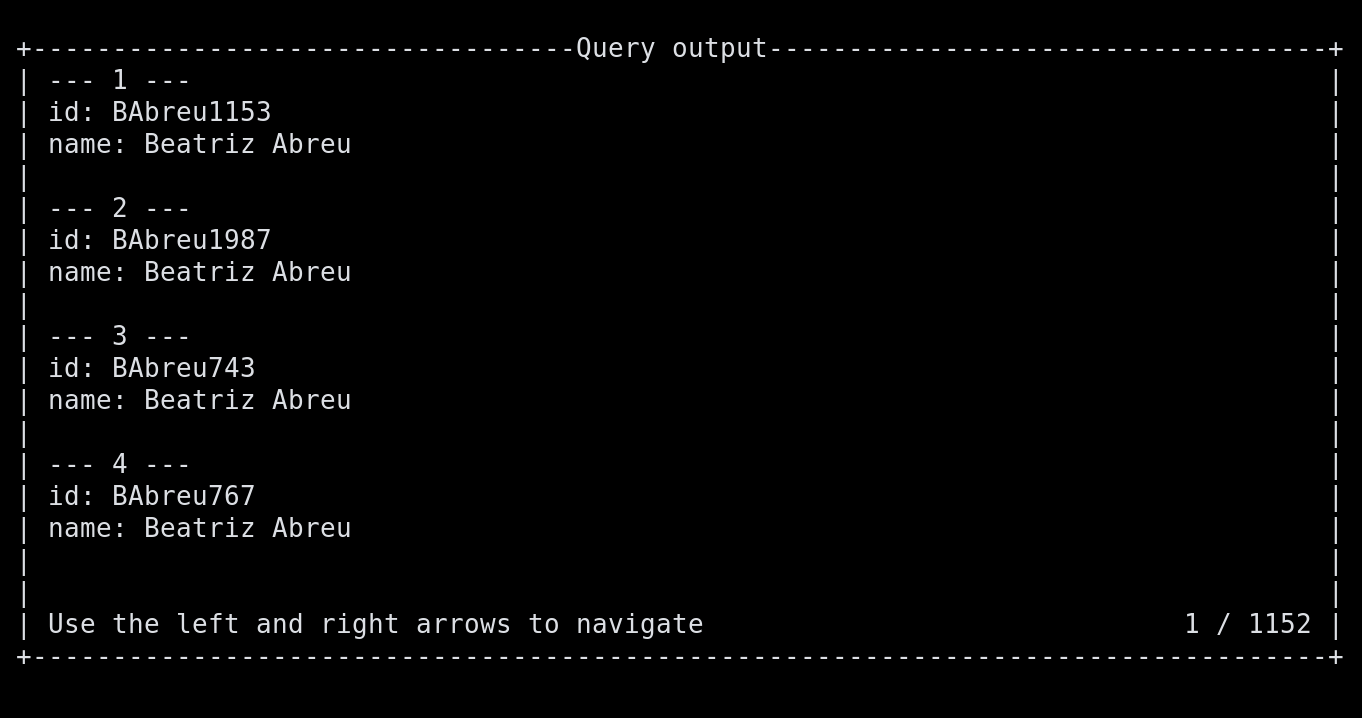
\includegraphics[scale=0.25]{res-fase2/interactive_screenshots/paging.png}
    \caption{Output paginado de uma \emph{query} (\texttt{activity\_paging})}
    \label{fig:paging}
\end{figure}

\begin{figure}[H]
    \centering
    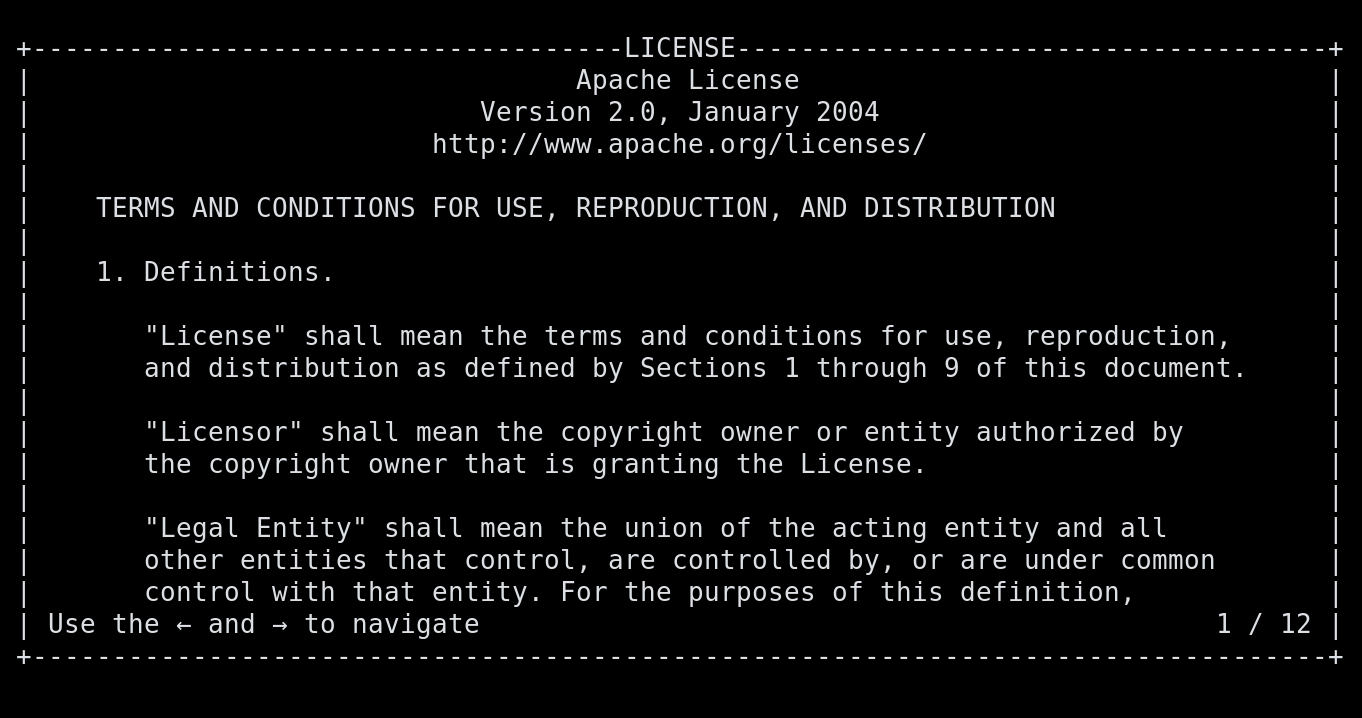
\includegraphics[scale=0.25]{res-fase2/interactive_screenshots/license.png}
	\caption{Licença da aplicação (\texttt{activity\_license})}
    \label{fig:license}
\end{figure}

\begin{figure}[H]
    \centering
    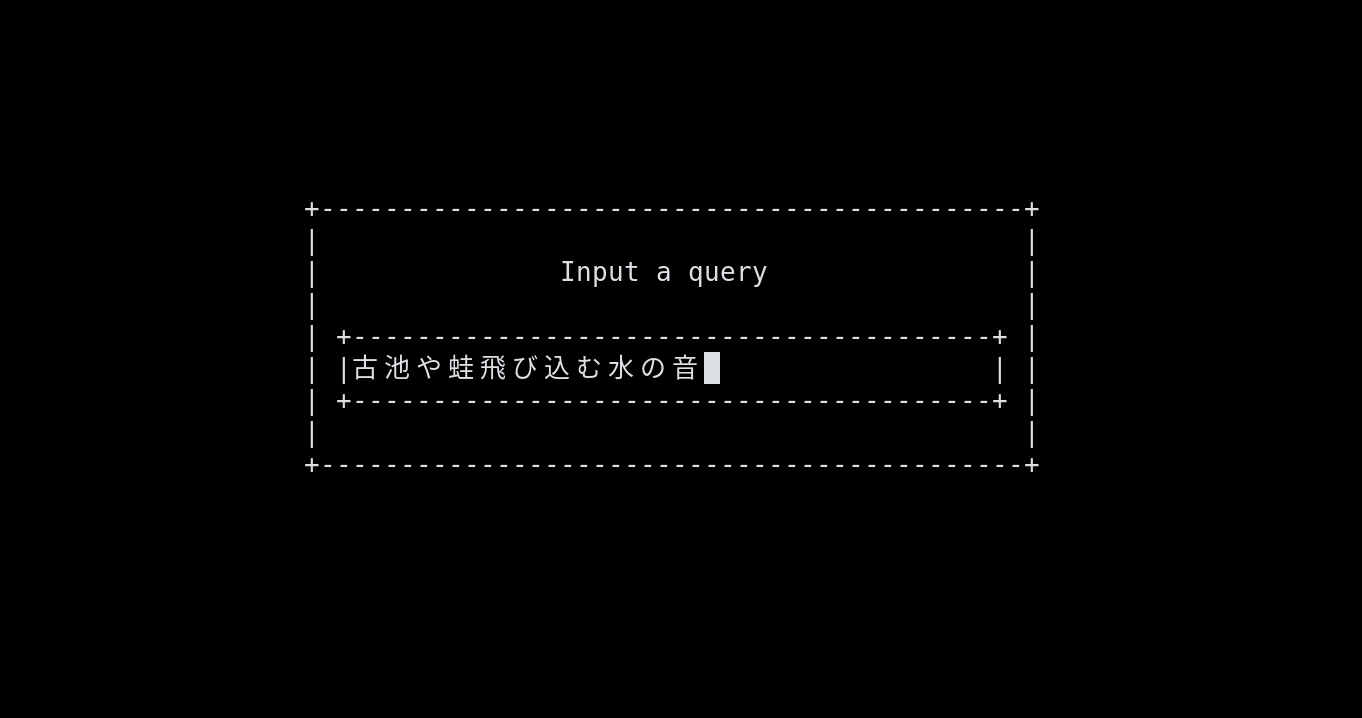
\includegraphics[scale=0.25]{res-fase2/interactive_screenshots/japanese.png}
    \caption{Suporte para caracteres de largura dupla numa \texttt{activity\_textbox}.
             O \emph{scrolling} mantém-se funcional.}
    \label{fig:japanese}
\end{figure}

\begin{figure}[H]
    \centering
    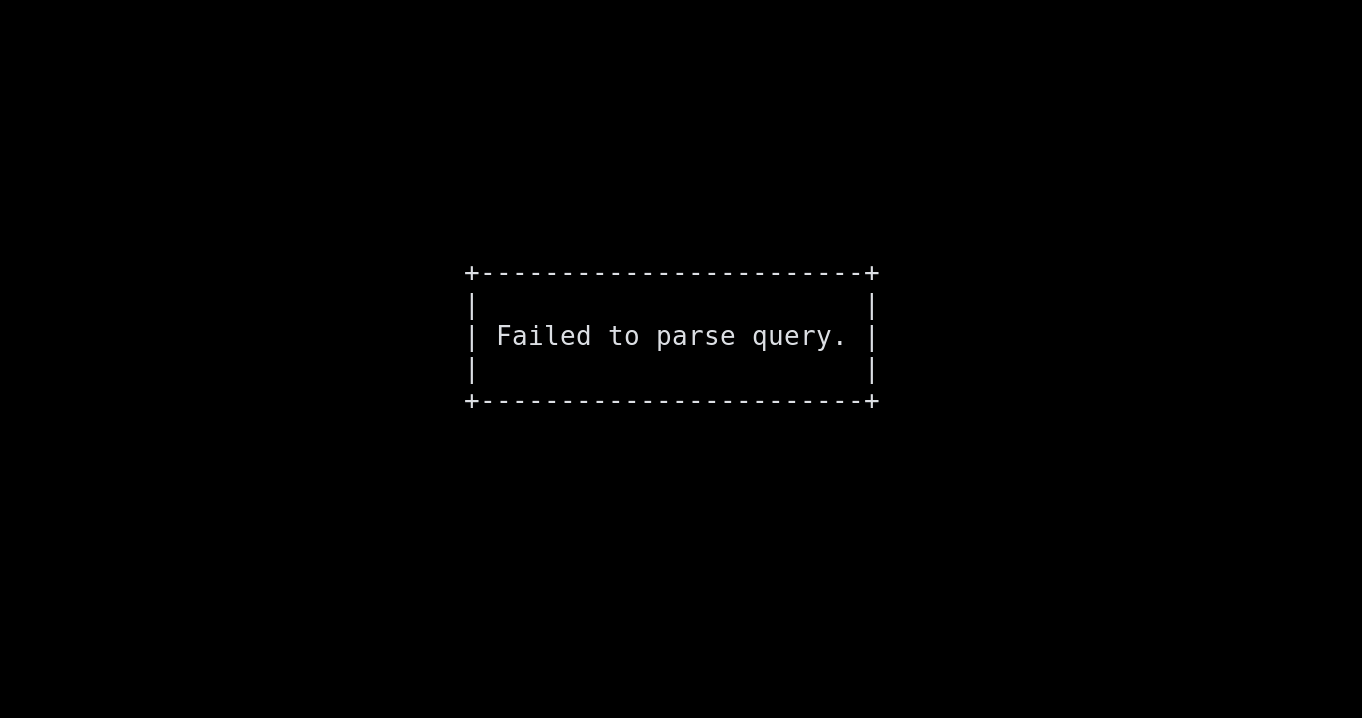
\includegraphics[scale=0.25]{res-fase2/interactive_screenshots/messagebox.png}
    \caption{Aviso de erro numa \texttt{activity\_messagebox}}
    \label{fig:messagebox}
\end{figure}

\subsection{\emph{Screenshots} do \emph{output} dos testes}
\label{sec:testing-screenshots}

\begin{figure}[H]
    \centering
    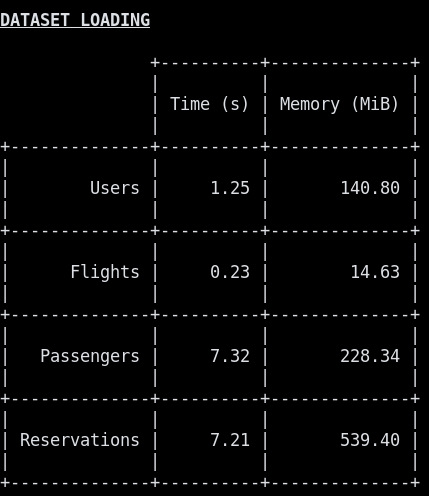
\includegraphics[scale=0.4]{res-fase2/testing_screenshots/dataset.png}
    \caption{Tabela de tempos de leitura de cada parte de um \emph{dataset}}
    \label{fig:dataset-screenshot}
\end{figure}

\begin{figure}[H]
    \centering
    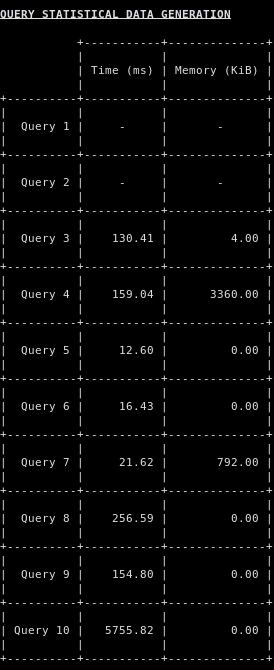
\includegraphics[scale=0.6]{res-fase2/testing_screenshots/statistics.png}
    \caption{Tabela de tempos de geração de dados estatísticos para cada \emph{query}}
    \label{fig:query-screenshot}
\end{figure}

\begin{figure}[H]
    \centering
    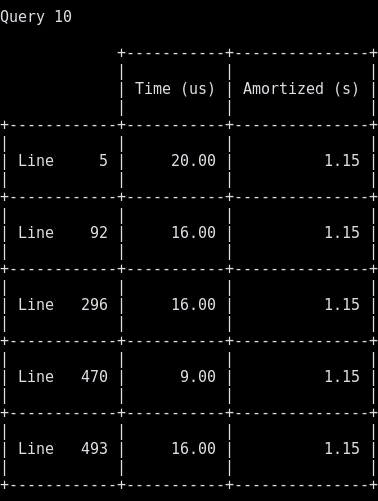
\includegraphics[scale=0.5]{res-fase2/testing_screenshots/query.png}
    \caption{Tabela de tempos de execução de cada \emph{query}. É visível como são automaticamente
             escolhidas duas unidades diferentes para as duas colunas.}
    \label{fig:q10-screenshot}
\end{figure}

\begin{figure}[H]
    \centering
    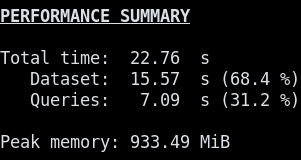
\includegraphics[scale=0.7]{res-fase2/testing_screenshots/summary.png}
    \caption{Sumário do \emph{benchmarking} da aplicação}
    \label{fig:performance-summary}
\end{figure}

\begin{figure}[H]
    \centering
    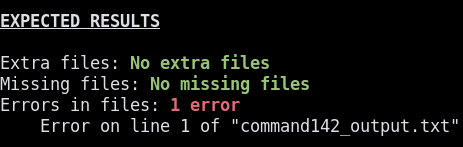
\includegraphics[scale=0.6]{res-fase2/testing_screenshots/diff.png}
    \caption{Exemplo de resultado de testes funcionais com um erro}
    \label{fig:diff-screenshot}
\end{figure}

\end{document}
